\documentclass{article}
\usepackage[utf8]{inputenc}
\author{Kevin L}

\usepackage{amsmath,amsthm,amssymb,amsfonts,graphicx,framed,indentfirst}
\usepackage[normalem]{ulem}
\usepackage[italicdiff]{physics}
\usepackage[T1]{fontenc}
%\usepackage{pifont} %For unusual symbols
%\usepackage{mathdots} %For unusual combinations of dots
\usepackage{wrapfig}
\usepackage{lmodern,mathrsfs}
\usepackage[inline,shortlabels]{enumitem}
\setlist{topsep=2pt,itemsep=2pt,parsep=0pt,partopsep=0pt}
\usepackage[dvipsnames]{xcolor}
\usepackage[utf8]{inputenc}
\usepackage[a4paper, top=0.5in,bottom=0.2in, left=0.5in, right=0.5in, footskip=0.3in, includefoot]{geometry}
\usepackage[most]{tcolorbox}
\usepackage{tikz,tikz-3dplot,tikz-cd,tkz-tab,tkz-euclide,pgf,pgfplots}
\pgfplotsset{compat=newest}
\usepackage{multicol}
\usepackage[bottom,multiple]{footmisc} %ensures footnotes are at the bottom of the page, and separates footnotes by a comma if they are adjacent
% \usepackage[backend=bibtex,style=numeric]{biblatex}
% \renewcommand*{\finalnamedelim}{\addcomma\addspace} % forces authors' names to be separated by comma, instead of "and"
% \addbibresource{bibliography}
\usepackage{hyperref}
\usepackage[nameinlink]{cleveref} %nameinlink ensures that the entire element is clickable in the pdf, not just the number
\usetikzlibrary{positioning}
\newcommand{\ep}{\varepsilon}
\newcommand{\N}{\mathbb{N}}
\newcommand{\Q}{\mathbb{Q}}
\newcommand{\R}{\mathbb{R}}
\newcommand{\C}{\mathbb{C}}
\newcommand{\Z}{\mathbb{Z}}
\renewcommand{\iff}{\Leftrightarrow}
\newcommand{\dom}{\text{dom }}
\DeclareMathOperator{\range}{\text{range}}
\usepackage{mathtools}
\DeclarePairedDelimiter\ceil{\lceil}{\rceil}
\DeclarePairedDelimiter\floor{\lfloor}{\rfloor}

\newtheoremstyle{mystyle}{}{}{}{}{\sffamily\bfseries}{.}{ }{}
\newtheoremstyle{cstyle}{}{}{}{}{\sffamily\bfseries}{.}{ }{\thmnote{#3}}
\makeatletter
\renewenvironment{proof}[1][\proofname] {\par\pushQED{\qed}{\normalfont\sffamily\bfseries\topsep6\p@\@plus6\p@\relax #1\@addpunct{.} }}{\popQED\endtrivlist\@endpefalse}
\makeatother

\theoremstyle{mystyle}{\newtheorem{definition}{Definition}[section]}
\theoremstyle{mystyle}{\newtheorem{proposition}[definition]{Proposition}}
\theoremstyle{mystyle}{\newtheorem{theorem}[definition]{Theorem}}
\theoremstyle{mystyle}{\newtheorem{lemma}[definition]{Lemma}}
\theoremstyle{mystyle}{\newtheorem{corollary}[definition]{Corollary}}
\theoremstyle{mystyle}{\newtheorem*{remark}{Remark}}
\theoremstyle{mystyle}{\newtheorem*{remarks}{Remarks}}
\theoremstyle{mystyle}{\newtheorem*{example}{Example}}
\theoremstyle{mystyle}{\newtheorem*{examples}{Examples}}
\theoremstyle{definition}{\newtheorem*{exercise}{Exercise}}
\theoremstyle{cstyle}{\newtheorem*{cthm}{}}
\theoremstyle{cstyle}{\newtheorem*{clemma}{}}

\tcolorboxenvironment{definition}{boxrule=0pt,boxsep=0pt,colback={red!10},left=8pt,right=8pt,enhanced jigsaw, borderline west={2pt}{0pt}{red},sharp corners,before skip=10pt,after skip=10pt,breakable}
\tcolorboxenvironment{proposition}{boxrule=0pt,boxsep=0pt,colback={Orange!10},left=8pt,right=8pt,enhanced jigsaw, borderline west={2pt}{0pt}{Orange},sharp corners,before skip=10pt,after skip=10pt,breakable}
\tcolorboxenvironment{theorem}{boxrule=0pt,boxsep=0pt,colback={blue!10},left=8pt,right=8pt,enhanced jigsaw, borderline west={2pt}{0pt}{blue},sharp corners,before skip=10pt,after skip=10pt,breakable}
\tcolorboxenvironment{lemma}{boxrule=0pt,boxsep=0pt,colback={Cyan!10},left=8pt,right=8pt,enhanced jigsaw, borderline west={2pt}{0pt}{Cyan},sharp corners,before skip=10pt,after skip=10pt,breakable}
\tcolorboxenvironment{corollary}{boxrule=0pt,boxsep=0pt,colback={violet!10},left=8pt,right=8pt,enhanced jigsaw, borderline west={2pt}{0pt}{violet},sharp corners,before skip=10pt,after skip=10pt,breakable}
\tcolorboxenvironment{proof}{boxrule=0pt,boxsep=0pt,blanker,borderline west={2pt}{0pt}{CadetBlue!80!white},left=8pt,right=8pt,sharp corners,before skip=10pt,after skip=10pt,breakable}
\tcolorboxenvironment{remark}{boxrule=0pt,boxsep=0pt,blanker,borderline west={2pt}{0pt}{Green},left=8pt,right=8pt,before skip=10pt,after skip=10pt,breakable}
\tcolorboxenvironment{remarks}{boxrule=0pt,boxsep=0pt,blanker,borderline west={2pt}{0pt}{Green},left=8pt,right=8pt,before skip=10pt,after skip=10pt,breakable}
\tcolorboxenvironment{example}{boxrule=0pt,boxsep=0pt,blanker,borderline west={2pt}{0pt}{Black},left=8pt,right=8pt,sharp corners,before skip=10pt,after skip=10pt,breakable}
\tcolorboxenvironment{examples}{boxrule=0pt,boxsep=0pt,blanker,borderline west={2pt}{0pt}{Black},left=8pt,right=8pt,sharp corners,before skip=10pt,after skip=10pt,breakable}
\tcolorboxenvironment{cthm}{boxrule=0pt,boxsep=0pt,colback={blue!10},left=8pt,right=8pt,enhanced jigsaw, borderline west={2pt}{0pt}{blue},sharp corners,before skip=10pt,after skip=10pt,breakable}
\tcolorboxenvironment{clemma}{boxrule=0pt,boxsep=0pt,colback={Cyan!10},left=8pt,right=8pt,enhanced jigsaw, borderline west={2pt}{0pt}{Cyan},sharp corners,before skip=10pt,after skip=10pt,breakable}

\usepackage[explicit]{titlesec}
\titleformat{\section}{\fontsize{24}{30}\sffamily\bfseries}{\thesection}{20pt}{#1}
\titleformat{\subsection}{\fontsize{16}{18}\sffamily\bfseries}{\thesubsection}{12pt}{#1}
\titleformat{\subsubsection}{\fontsize{10}{12}\sffamily\large\bfseries}{\thesubsubsection}{8pt}{#1}

\titlespacing*{\section}{0pt}{5pt}{5pt}
\titlespacing*{\subsection}{0pt}{5pt}{5pt}
\titlespacing*{\subsubsection}{0pt}{5pt}{5pt}

\newcommand{\Disp}{\displaystyle}
\newcommand{\qe}{\hfill\(\bigtriangledown\)}
\DeclareMathAlphabet\mathbfcal{OMS}{cmsy}{b}{n}
\setlength{\parindent}{0.2in}
\setlength{\parskip}{0pt}
\setlength{\columnseprule}{0pt}

\definecolor{contcol1}{HTML}{72E094}
\definecolor{contcol2}{HTML}{24E2D6}
\definecolor{convcol1}{HTML}{C0392B}
\definecolor{convcol2}{HTML}{8E44AD}

\usepackage{setspace}
\setstretch{1.25}

\pgfplotsset{soldot/.style={color=black,only marks,mark=*},
  holdot/.style={color=black,fill=white,only marks,mark=*},
compat=1.12}

\counterwithin*{equation}{section}
\counterwithin*{equation}{subsection}

\renewcommand{\epsilon}{\varepsilon}


\begin{document}
\title{MATH 1052 Notes}
\date{Winter Term 1 2022}
\maketitle

\begin{tcolorbox}[title=, fonttitle=\huge\sffamily\bfseries\selectfont,interior style={left color=contcol1!40!white,right color=contcol2!40!white},frame style={left color=contcol1!80!white,right color=contcol2!80!white},coltitle=black,top=2mm,bottom=2mm,left=2mm,right=2mm,drop fuzzy shadow,enhanced,breakable]
\tableofcontents
\end{tcolorbox}


\newpage
\section{Infinite Series}
\begin{cthm}[Theorem 14.6]
The \textbf{Comparison Test} \newline
Let $\sum{a_n}$ be a series of non-negative terms.
\begin{enumerate}
    \item If $\sum{a_n}$ converges and $\forall n \;|b_n| \leq a_n $, then $b_n$ converges.
    \item If $\sum{a_n} = \infty$ and $\forall n \; b_n \geq a_n$, then $\sum{b_n} = \infty$.
\end{enumerate}
\end{cthm}
\begin{proof}
\textbf{Case 1:} \newline
Let $s_n = \sum_{k=1}^n a_k$ and $t_n = \sum_{k=1}^n b_k$ be the sequence of partial sums. Since $\sum a_n$ converges, $s_n$ converges, so $s_n$ is a Cauchy sequence.

Thus, let $\ep > 0$ be given. Then, $\exists N$ s.t. $n, m > N \implies |s_n - s_m| < \ep$.
We take $n > m$. Then,
\begin{align*}
    |t_n - t_m| &= \left|\sum_{k = m+1}^n b_k\right|\\
    &\leq \sum_{k=m+1}^n |b_k| \tag{By Triangle Inequality}\\
    &\leq \sum_{k=m+1}^n a_k\\
    &= |s_n - s_m| < \ep\\
\end{align*}
Hence $(t_n)$ is Cauchy, and so converges, therefore $\sum b_n$ converges.
\newline
\textbf{Case 2:}\newline
With $s_n$ and $t_n$ as above, we have
\begin{align*}
    t_n &= \sum_{k=1}^n b_k\\
    &\geq \sum_{k=1}^n a_k\\
    &= s_n\\
\end{align*}
Since $\sum a_n = \infty$, $\lim s_n = \infty$, then by Exercise 9.9a), $\lim t_n = \infty$. Thus, $\sum b_n = \infty$.
\end{proof}

\begin{proposition}
If $\sum a_n$ converges, then $\sum ka_n = k \sum a_n$. \newline
If $\sum a_n$ diverges, and $k \not = 0$, then $\sum ka_n$ diverges.
\end{proposition}

\begin{examples}
Consider \[\sum_{k=1}^\infty \frac{2n+1}{3n^2 + n}\]
By rough intuition, this is roughly equal to $\frac{1}{n}$, which diverges.
We have
\begin{align*}
    \frac{2n+1}{3n^2+n} &> \frac{2n}{4n^2}\\
    &= \frac{2}{n}\\
    &> \frac{1}{n}
\end{align*}
Since $\sum \frac{1}{n}$ diverges, by the comparison test this series diverges.
\newline
Consider \[\sum_{k=1}^\infty \frac{2n+1}{3n^3 + n}\]
We have\
\begin{align*}
    \frac{2n+1}{3n^3} &< \frac{2n+n}{3n^3}\\
    &= \frac{1}{n^2}\\
\end{align*}
Since $\sum\frac{1}{n^2}$ converges, by the comparison test this series converges.
\end{examples}
\begin{definition}
A series $\sum a_n$ \textbf{converges absolutely} if $\sum |a_n|$ converges.
If $\sum a_n$ converges, but $\sum |a_n|$ diverges, then $\sum a_n$ \textbf{converges conditionally}.
\end{definition}
\begin{cthm}[Theorem 14.7]
Absolutely convergent series are convergent.
\end{cthm}
\begin{proof}
Suppose $\sum |a_n|$ is convergent. Since $|a_n| \leq |a_n|$, and $|a_n|$ converges, then $|a_n|$ converges by the comparison test.
\end{proof}
\begin{examples}
Consider \[\sum_{n=1}^\infty \frac{(-1)^n}{n^2}\] Since $\sum \left| \frac{(-1)^n}{n^2} \right| = \sum \frac{1}{n^2}$ is a convergent series, this series converges absolutely.
\newline
Consider \[\sum_{n=1}^\infty \frac{(-1)^{n+1}}{n}\]
Since the absolute value of this expression is equal to $\frac{1}{n}$, then this series does not converge absolutely. However, since this is an alternating sequence this series does converge conditionally.
\end{examples}
\begin{proposition}
If $\sum a_n$ converges, then $\sum ka_n = k \sum a_n$. \newline
If $\sum a_n$ and $\sum b_n$ converge absolutely, then
\[\sum (a_n + b_n) = \sum a_n + \sum b_n\]
\end{proposition}
\begin{example}
Consider
\begin{align*}
    \sum_{n=2}^\infty \frac{4^{n+1}}{5^n} &= 4 \sum_{n=2}^\infty \frac{4^n}{5^n}\\
    &=4 \sum_{n=2}^\infty (\frac{4}{5})^n\\
    &= 4(\frac{4}{5})^2 \sum_{n=2}^\infty (\frac{4}{5})^{n-2}\\
    \text{Let } m &= n - 2\\
    &= 4(\frac{4}{5})^2 \sum_{m=0}^\infty (\frac{4}{5})^{m}\\
    &= 4(\frac{4}{5})^2 (\frac{1}{1 - \frac{4}{5}})\\
\end{align*}
An alternative way to solve this is
\begin{align*}
    4 \sum_{n=2}^\infty (\frac{4}{5}) &= 4\left( \sum_{n=0}^\infty (\frac{4}{5})^n - \sum_{n=0}^1 (\frac{4}{5})^n\right)\\
    &= 4\left( \sum_{n=0}^\infty (\frac{4}{5})^n - 1 - \frac{4}{5}\right)\\
    &= 4\left( \frac{1}{1 - \frac{4}{5}} - 1 - \frac{4}{5}\right)\\
    \end{align*}
\end{example}
\begin{cthm}[Theorem 14.8] The \textbf{Ratio Test} \newline
Let $\sum a_n$ be a series of non-zero terms for which \[L = \left|\frac{a_{n+1}}{a_n}
\right| \] exists. \newline Then, 
\[\sum a_n
\begin{cases}
    \text{converges absolutely},    \text{if $L < 1$}\\
    \text{diverges},    \text{if $L > 1$}\\
    \text{can either converge or diverge},    \text{if $L = 1$}\\
\end{cases}
\]
\end{cthm}
\begin{proof}
Since $\left|\frac{a_{n+1}}{a_n}\right| > 0$, we have $L \geq 0$ (by Textbook exercise 9.9c)
\newline
\textbf{Case 1:}\newline
Since $0 \leq L < 1$,  we can choose $k$ such that $0 \leq l < k < 1$ by Theorem 4.7. Thus, $k-L >0$. Therefore, $\exists N$ s.t. \[n > N \implies \left| |\frac{a_{n+1}}{a_n}| - L \right| < k - L\]
Thus, $-(k-L) < \left| \frac{a_{n+1}}{a_n}\right| < k - L $ and so $\left| \frac{a_{n+1}}{a_n}\right| < k$. Therefore, $|a_{n+1}| < k|a_n|$. Hence, $|a_{N+2}| < k|a_{N+1}|$ (Recall this holds for $n > N$ from the epsilon proof). \newline As a result, we also have $|a_{N+3}| < k|a_{N+2}| < k^2|a_{N+1}|$ and so on. Thus in general, we have $|a_{N+j}| < k^{j-1}|a_{N+1}|$ for some $j \in \N$ with $j \geq 2$. Therefore, we have 
\begin{align*}
    \sum_{j=2}^\infty k^{j-1}|a_{N+1}| &= |a_{N+1}| \sum_{j=2}^\infty k^{j-1}\\
    &= |a_{N+1}|\frac{1}{k} \sum_{j=2}^\infty k^j
\end{align*}
This is a convergent series since $0 < k < 1$.
Thus by the comparison test, $\sum a_n$ converges absolutely.
\newline
\textbf{Case 2:}\newline
Since $L > 1$, we can choose $1 < k < L$. Then $L - k > 0$.
Therefore, $\exists N$ s.t. \[n > N \implies \left| |\frac{a_{n+1}}{a_n}| - L \right| < L-k\]
Thus, $-(L-k) < \left| \frac{a_{n+1}}{a_n}\right| < L-k $ and so $k < \left| \frac{a_{n+1}}{a_n}\right|$. Therefore, $|a_{n+1}| > k|a_n|$. Thus in general, we have $|a_{N+j}| > k^{j-1}|a_{N+1}|$ for some $j \in \N$ with $j \geq 2$.
Since $\lim k^{j-1}|a_{N+1}| = |a_{N+1}| \frac{1}{k} \lim_{j\to\infty} k^j = \infty$, by Exercise 9.9a, $\lim |a_n| = \infty$, thus $\lim a_n \not = 0$. Thus this sequence diverges.
\end{proof}
\begin{example}
Consider \[\sum_{n=1}^\infty \frac{n^2}{2^n}\]
We have
\begin{align*}
    \lim_{n\to\infty} \left|\frac{\frac{(n+1)^2}{2^{n+1}}}{\frac{n^2}{2^n}}\right|  &= \lim_{n\to\infty} \left| (\frac{n+1}{n})^2 (\frac{2^n}{2^{n+1}})\right|\\
    &= \frac{1}{2} \lim \left(\frac{n+1}{n}\right)^2\\
    &= \frac{1}{2}\\
\end{align*}
Since $0 < \frac{1}{2} < 1$, this series is convergent.
\end{example}

\begin{cthm}[Theorem 14.9] The \textbf{Root Test}\newline
Let $\sum a_n$ be a series for which $L = \lim |a_n|^\frac{1}{n}$ exists. Then,\[\sum a_n
\begin{cases}
    \text{converges absolutely},    \text{if $L < 1$}\\
    \text{diverges},    \text{if $L > 1$}\\
    \text{can either converge or diverge},    \text{if $L = 1$}\\
\end{cases}
\]
\end{cthm}
\begin{proof}
\textbf{Case 1:}\newline
Since $0 \leq L < 1$,  we can choose $k$ such that $0 \leq l < k < 1$ by Theorem 4.7. Thus, $k-L >0$. Therefore, $\exists N$ s.t. \[n > N \implies \left| |a_n|^\frac{1}{n} - L \right| < k - L\]
Thus, $-(k-L) < |a_n|^\frac{1}{n} < k - L $ and so $|a_n|^\frac{1}{n} < k$. This is equal to $|a_n| < k^n$. Since $0 < k < 1$, $\sum k^n$ is convergent. Thus by the comparison test, $|a_n|$ is also convergent.\newline
\textbf{Case 2:}\newline
Since $L > 1$, we can choose $1 < k < L$. Then $L - k > 0$.
Therefore, $\exists N$ s.t. \[n > N \implies \left| |a_n|^\frac{1}{n} \right| < L-k\]
Thus, $-(L-k) < |a_n|^\frac{1}{n} < L-k $ and so $k < |a_n|^\frac{1}{n}$. Therefore, $|a_{n}| > k^n$. Since $k > 1$, $\sum k^n$ is divergent. Thus by the comparison test, $|a_n|$ is divergent.
\end{proof}
\begin{example}
Consider \[\sum_{n=0}^\infty \frac{(-1)^n n^{2n}}{2^n (n^2+1)^n}\]
We have
\begin{align*}
    \sum_{n=0}^\infty \frac{(-1)^n n^{2n}}{2^n (n^2+1)^n}&= \sum \left(\frac{-1 \cdot n^2}{2 \cdot (n^2+1)}\right)^n\\
    \text{Since } \lim \left|\left(\frac{-1 \cdot n^2}{2 \cdot (n^2+1)}\right)^n\right|^\frac{1}{n} &= \lim \frac{n^2}{2n^2+2}\\
    &= \frac{1}{2}\\
\end{align*}
Since $\frac{1}{2} < 1$, this converges.
\end{example}
\begin{cthm}[Theorem 15.3]
The \textbf{Alternating Series Test} \newline
If $(a_n)$ is a decreasing sequence of non-negative terms and has a limit of $0$, then the alternating series $\sum (-1)^{n+1} a_n$ converges.
\end{cthm}
\begin{proof}
Let $s_n$ be the series of partial sums, or \[s_n = \sum_{k=1}^n (-1)^{k+1} a_k 
\]
Then, $s_n$ converges $\iff$ $(a_n)$ converges.

Consider the subsequence $s_{2n}$, which is all the even terms.
Then \begin{align*}
    &S_{2(n+1)} - S_{2n} \tag{Every term except for $n+1$ and $n+2$ cancels out} \\ &= -a_{2n+2} + a_{2n+1} \tag{$(-1)^{n+1}$ is negative for $n=2$, but positive for $n=1$}\\
    &-a_{2n+2} + a_{2n+1} \geq 0 \tag{$(a_n)$ is decreasing}\\
\end{align*}
Thus, because $(a_n)$ is decreasing, $(s_{2n})$ is increasing.

Consider the subsequence $s_{2n+1}$, which is all the odd terms.
Then \begin{align*}
    S_{2(n+1)+1} - S_{2n+1}  &= a_{2n+3} - a_{2n+2}\\ 
    -a_{2n+2} + a_{2n+1} &\leq 0 \tag{$(a_n)$ is decreasing}\\
\end{align*}
Thus, because $(a_n)$ is decreasing, $(s_{2n+1})$ is decreasing.

We now prove that \begin{equation}
s_{2m} \leq s_{2n+1} \;\forall m, n \in \N.\end{equation}
Since $s_{2m+1} - s_{2n} = a_{2n+1} \geq 0$, we have $s_{2n} \leq s_{2n+1}$.

If $m \leq n$, then $s_{2m} \leq s_{2n}$ (Since even subsequences are increasing), so $s_{2m} \leq s_{2n+1}$ by transitivity.

If $m > n$, then $s_{2n+1} \geq s_{2m+1}$ (Since odd subsequences are decreasing), so $s_{2n+1} \geq s_{2m}$ Thus, $(1)$ holds.

Therefore, $(s_{2n})$ is increasing, but it's bounded above by any odd partial sum $(1)$, and bounded below by its first term. Thus, $s_{2n}$ is convergent to some $s$.

Therefore, $(s_{2n+1})$ is decreasing, but it's bounded above by its first term, and bounded below by any even partial sum $(1)$. Thus, $s_{2n+1}$ is convergent to some $t$.    

We have
\begin{align*}
    t - s &= \lim s_{2n+1} - \lim s_{2n}\\
    &= \lim (s_{2n+1} - s_{2n})\\
    &= \lim (a_{2n+1})\\
    &= 0 \tag{$\lim (a_n) = 0$ by def.}\\
\end{align*}
Thus $s = t$, and so both $s_{2n}$ and $s_{2n+1}$ is convergent to $s$. Thus, $\lim s_n = s$.

\end{proof}
\begin{example}
Consider \[\sum \left(\frac{(-1)^{n+1}}{n}\right)\] Note that the limit of this sequence is $0$, and the terms are decreasing. Then this series converges.
\end{example}
\begin{remark}
Note that in the above series, the absolute value of the sequence, which is $\frac{1}{n}$ diverges, so this series only converges conditionally.
As an aside, the above series converges to $\ln 2$.
\end{remark}

\section{Functions}
\begin{definition}
A \textbf{function} $f: A \to B$ is a relation from $A$ to $B$ where each element of $A$ maps to exactly one element in $B$, called $f(x)$. 

$A$ is called the \textbf{domain} of $f$, written $\dom(f)$.

$B$ is called the \textbf{co-domain} of $f$.

If no domain for $f$ is given, it is understood that it is the \textbf{natural domain}, the largest subset of the reals on which $f$ is defined.
\end{definition}
\begin{example}
The function $f$ defined by $f(x) = \frac{1}{x^2}$ has natural domain $\{x \in \R \mid x \not = 0 \}$.

The function $g$ defined by $g(x) = \sqrt{9-x^2}$ has natural domain \begin{align*}
    9 - x^2 &\geq 0\\
    9 &\geq x^2\\
    3 &\geq |x|\\
\end{align*}
$\{x \in \R \mid -3 \leq x \leq 3 \}$ or $[-3, 3]$.
\end{example}
\begin{definition}
Let $f$ be a real-valued function with $\dom(f) \subseteq \R$ and let $a \in \R$ be the limit of some sequence in the domain. Let $L \in \R$.
Then, $\lim_{x\to a} = L$ iff $\forall \ep > 0$, there is $\delta > 0$ such that $x \in \dom(f)$ and $0 < \abs{x -a} < \delta \implies \abs{f(x) - L} < \ep$.

i.e. We can bring $f(x)$ arbitrarily close to $L$ (within $\ep$) by taking $x$ close enough to $a$ (within $\delta$).
\end{definition}
\begin{examples}
Prove \[\lim_{x\to 4}(5x-3) = 17 \]

Given $\ep > 0$, find $\delta$ > 0 such that $x \in \R$ and \[0 < \abs{x - 4} < \delta \implies |5x-3-17| < \ep\]

Note that \begin{align*}
    |5x-3-17| &= |5x-20|\\
    &= 5|x-4|\\
    &< 5\delta\\
    &\leq \ep\\
\end{align*}
Thus, we can choose delta as $\frac{\ep}{5}$.

Therefore, let $\ep > 0$ be given and $\delta = \frac{\ep}{5} $. Then $x \in \R$ and $0 < |x-4| < \delta \implies$
\begin{align*}
    |5x-3-17| &= 5|x-4|\\
    &< 5\delta\\
    &= \ep\\
\end{align*}
as required. \qed


Prove \[
\lim_{x\to 2}(3x^2-1) = 11
\]
Note that $\dom(f) = \R$.

Given $\ep > 0$, find $\delta > 0$ such that $0 < \abs{x-2} < \delta \implies \abs{3x^2 - 1 - 11} < \ep$.

Rough Work:
We have 
\begin{align*}
    \abs{3x^2 - 1 - 11} &= 3\abs{x^2-4}\\
    &= 3|x-2||x+2|\\
\end{align*}
We get to choose $\delta$, so choose it such that $\delta < 1$.

Then, \begin{align*}
    |x-2| &< 1\\
    &\implies -1 < x-2 < 1\\
    &\implies 3 < x + 2 < 5\\
    &\implies |x+2| < 5\\
\end{align*}

Another way to show is is to use the triangle inequality.
\begin{align*}
    |x+2| &= |x-2 + 4|\\
    &\leq |x-2| + 4\\
    &< 1 + 4\\
    &= 5\\
\end{align*}

Thus, \begin{align*}
    3|x-2||x+2| &< 15 |x-2| \tag{Provided $\delta < 1$}\\
    &< 15\delta \tag{We want this expression to be $\leq \ep$}\\
\end{align*}

Take $\delta \leq \frac{\ep}{15}$, or $\delta = \min(\frac{\ep}{15}, 1)$.

Proof:
Let $\ep > 0$ be given. Choose $\delta = \min(\frac{\ep}{15}, 1)$. Then, $x \in \R$ and $0 < |x-2| < \delta$ implies both
\begin{align*}
    |x-2| < 1 &\implies -1 < x-2 < 1\\
    &\implies 3 < x+2 < 5\\
    &\implies |x+2| < 5\\
\end{align*}
and \[
|x-2| < \delta \implies |x-2| < \frac{\ep}{15}
\]
We then have
\begin{align*}
    |3x-1-11| &= 3 \abs{x-2}\abs{x+2}\\
    &< 3(\frac{\ep}{15})(5)\\
    &= \ep\\
\end{align*}
\qed

\textbf{Example 3:}\newline
Let \[
f(x) = \begin{cases}
    2x, &\text{ if } x \not= 1\\
    5, &\text{ if } x=1\\
\end{cases}
\]
\begin{center}
\begin{tikzpicture}
\begin{axis}[
    axis lines = left,
    % xlabel = \(x\),
    % ylabel = {\(f(x)\)},
    axis lines=middle,
    axis line style={->},
    ylabel near ticks,
    xlabel near ticks,
]
\addplot [
    domain=-2:2, 
    samples=100, 
    color=red,
    style=thick,
]
{2*x};

\addplot[holdot] coordinates{(1,2)};
\addplot[soldot] coordinates{(1,5)};
\end{axis}
\end{tikzpicture}
\end{center}

Note that $|x-1| > 0 \implies x \not= 1$.

Thus, \begin{align*}
    |f(x) - 2| &= |2x-2|\\
    &= 2|x-1|\\
    &< 2\delta\\
    (& \leq \ep)\\
\end{align*}
Choose $\delta = \frac{\ep}{2}$.

Proof:
Let $\ep > 0$ be given, choose $\delta = \frac{\ep}{2}$. Then, $x \in \R$ and $0 < |x-1| < \delta \implies$
\begin{align*}
    |f(x)-2| &= |2x-2| \tag{$x \not = 1$}\\
    &= 2|x-1|\\
    &< 2\delta\\
    &= 2 \cdot \frac{\ep}{2}\\
    &= \ep\\
\end{align*}
\qed

\textbf{Example 4:}\newline
Let \[
f(x) = \frac{x^2-1}{x-1}
\]
Prove $\lim_{x\to 1} f(x) = 2$.
The domain of $f$ is $\{x \in \R \mid x \not = 1\}$.

Note that $\frac{x^2-1}{x-1} = x+1$ if $x\not=1$.

Given $\ep > 0$, find $\delta > 0$ such that $x\in \dom(f)$ and $0 < |x-1| < \delta \implies |f(x) - 2| < \ep$.

Since $x \not = 1$, 
\begin{align*}
    |f(x)-2| &= |\frac{x^2-1}{x-1} - 2|\\
    &= |x+1 - 2|\\
    &= |x-1|\\
    &< \delta\\
    (&\leq \ep)\\
\end{align*}
Choose $\delta = \ep$.

Proof:
Let $\ep > 0$ be given. Choose $\delta = \ep$. Then, $0 < |x-1| < \delta \implies x \not = 1$ .
We have \begin{align*}
    |f(x)-2| &= |\frac{x^2-1}{x-1} - 2|\\
    &= |x+1 - 2|\\
    &= |x-1|\\
    &< \delta\\
    &= \ep
\end{align*}
\qed
\end{examples}
\begin{definition}
Let $f$ be a real-valued function with $\dom(f) \subseteq \R$. Let $a \in \dom(f)$. Then $f$ is \textbf{continuous} at $a$ iff \[
\lim_{x\to a}f(x) = f(a)\]
If $f$ is continuous on each $a \in S$, for some $S \subseteq \dom(f)$, then $f$ is continuous on $S$.
\end{definition}
\begin{examples}
Let $f(x) = 5x-3$. We've proved that $\lim_{x\to 4} f(x) = 17$. Since $f(4) = 17$, $f$ is continuous at $x=4$.

Let $g(x) = 3x^2-1$. We've proved that $\lim_{x\to 2} g(x) = 11$. Since $g(2) = 11$, $g$ is continuous at $x=2$.

Let $h(x) = \begin{cases}
    2x, &\text{ if } x \not= 1\\
    5, &\text{ if } x=1\\
\end{cases}$. We've proved that $\lim_{x\to 1} h(x) = 2$. Since $h(1) = 5$, $h$ is discontinuous at $x=1$.

Let $k(x) = \frac{x^2-1}{x-1}$. Since $1 \not\in\dom(k)$, $k$ is discontinuous at $x=1$.

\textbf{Example 2:}

Let \[
f(x) = f(x) = \begin{cases}
    x \sin (\frac{1}{x}), &\text{ if } x \not= 0\\
    0, &\text{ if } x=0\\
\end{cases}
\]
\begin{center}
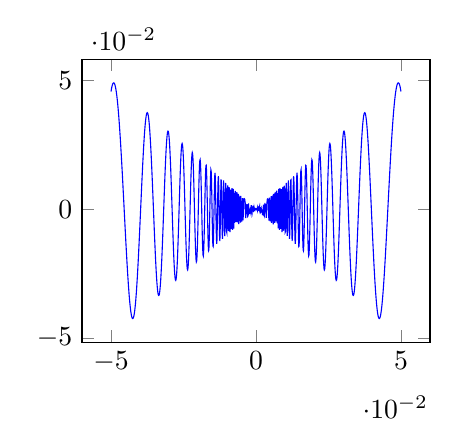
\begin{tikzpicture}
\begin{axis}[
 width=6cm,
%  axis lines=middle,
%  ticklabel style={fill=white},
%  xmin=-0.1,xmax=0.1,
%  ymin=-0.1,ymax=0.1,
]
\addplot[blue,samples=1000,domain=-0.05: 0.05]   {\x*sin(1/\x r)};
\end{axis}

\end{tikzpicture}
\end{center}

We prove that $f$ is continuous at $x=0$. We must show $\lim_{x\to 0} f(x)= f(0) = 0$.

Given $\ep > 0$, find $\delta$ such that \[
0 < |x-0| < \delta \implies |f(x) - 0| < \ep
\]
Note that $x > 0 \implies x \not = 0$.
Thus,  \begin{align*}
    |f(x)-0| &= |x\sin{\frac{1}{x}}|\\
    &= |x| |\sin{\frac{1}{x}}|\\
    &\leq |x| \tag{$|\sin{a}| \leq 1$}\\
    &< \delta\\
    (&\leq \ep)\\
\end{align*}
Choose $\delta = \ep$.

Let $\ep > 0$ be given. Choose $\delta = \ep$. Then $0 < |x| < \delta \implies x \not = 0$, so \[
|f(x)-0| = |x\sin{\frac{1}{x}}| \leq |x| < \delta = \ep
\]
\end{examples}
\begin{cthm}[Theorem 17.2]
Let $f$ be a real valued function with $\dom(f) \subseteq R$.
Let $a \in \dom(f)$. Then, $f$ is continuous at $a$ if and only if for every sequence $(x_n)$ in $\dom(f)$ converging to $a$, we have \[\lim_{n\to\infty} f(x_n) = f(a)\]
\end{cthm}
\begin{example}
Prove that $f(x) = 3x^3 - 2x^2 + x + 1$ is continuous on $\R$.

The old way to prove this would be to show that for an arbitrary element of $x_0 \in \R$, $\lim_{x\to x_0} f(x_0) = x_0$.

However, we can use Theorem 17.2.
Suppose \[
\lim_{n\to\infty}x_n = x_0
\]
Then, \begin{align*}
    \lim_{n\to\infty} f(x_n) &= \lim_{n\to\infty} (3x_n^3 - 2x_n^2 + x_n + 1)\\
    &= 3(\lim_{n\to\infty} x_n)^3 - 2(\lim_{n\to\infty}x_n)^2 + \lim_{n\to\infty} x_n + \lim_{n\to\infty} 1\\
    &= {3x_0}^3  -2{x_0}^2 +x_0 + 1\\
    &= f(x_0)\\
\end{align*}
\end{example}
\begin{proof}
We show the forwards direction. 

Suppose $f$ is continuous at $a$, and let $(x_n)$ be a sequence in the domain of $f$ with $\lim_{n\to\infty} x_n = a$. Then, we show \[\lim f(x_n) = f(a)\] 

Let $\ep > 0$ be given. Since $f$ is continuous at $a$, $\exists \delta > 0$ such that $x \in \dom(f)$ and \begin{equation}
    |x-a| < \delta \implies |f(x) - f(a)| < \ep.
\end{equation}
Since $\lim x_n = a$, there is $N$ such that $n > N \implies |x_n - a| < \delta$. (Take $\ep = \delta$)

Take $n > N$, then $|x_n - a| < \delta$ and so by (2) with $x = x_n \implies$
\[
|f(x_n) - f(a)| < \ep
\]
as required.

We show the reverse direction.
Suppose for any sequence $(x_n)$ in $\dom(f)$ convergent to $a$, \begin{equation}
    \lim_{n\to\infty} f(x_n) = f(a)
\end{equation}
but $f$ is not continuous. Then, $\exists \ep > 0$ such that $\forall \delta > 0$, the implication \[
x \in \dom(f) \text{ and } 0 < |x-a| < \delta \implies |f(x) - f(a)| < \ep
\]
is false. In particular, $\forall n \in \N$, $\exists x_n \in \dom(f)$ such that $0 < |x_n - a| < \frac{1}{n}$, but $|f(x) - f(a)| \geq \ep$.

Since $0 < |x_n - a| < \frac{1}{n}$ and $\lim \frac{1}{n} = 0$, by squeeze theorem $\lim (x_n - a) = 0$, so $\lim x_n = a$.

However, since $|f(x_n) - f(a) \geq \ep > 0$, $\lim f(x_n) \not = f(a)$, which contradicts (3). 
\end{proof}
\begin{definition}
Let $f, g$ be real valued functions and let $k \in \R$. Then, \[(kf)(x) = kf(x) \; \forall x \in \dom(f)\]

Then, \[(f + g)(x) = f(x) + g(x) \; \forall x \in \dom(f) \cap \dom(g)\]
Then, \[(fg)(x) = f(x)g(x) \; \forall x \in \dom(f) \cap \dom(g)\]
Then, \[(\frac{f}{g})(x) = \frac{f(x)}{g(x)} \; \forall x \in \dom(f) \cap \dom(g) \text{ and for where } g(x) \neq 0\]
\end{definition}
\begin{cthm}[Theorem 17.3 \& 17.4]
Let $f$ and $g$ be real valued functions continuous at $x_0$, and let $k \in \R$. Then the following are continuous at $x_0$.
\begin{itemize}
    \item $kf$
    \item $|f|$
    \item $f + g$
    \item $fg$
    \item $\frac{f}{g}$ if $g(x_0) \neq 0$
\end{itemize}
\end{cthm}
\begin{proof}
Let $(x_n)$ be a sequence in $\dom(f)$ with $\lim x_n = x_0$. Since $f$ is continuous at $x_0$, by theorem \[
\lim f(x_n) = f(x_0)
\]
Then, \[
\lim_{n\to\infty} kf(x_n) = k \lim f(x_n) = kf(x_0)
\]
Thus $kf$ is continuous at $x_0$.
\end{proof}
\begin{definition}
Let $f$, $g$ be real valued functions. Define the function $g \circ f$ ("g composed with f") by \[
(g \circ f)(x) = g(f(x))
\]
The domain is $x \in \dom(f) \cap f(x) \in \dom(g)$.
\end{definition}
\begin{example}
Let $f(x) = x + 1$, $g(x) = x^2$

\[
(g \circ f)(x) = g(f(x)) = g(x+1) = (x+1)^2
\]
\[
(f \circ g)(x) = f(g(x)) = f(x^2) = x^2 + 1
\]
\end{example}
\begin{cthm}[Theorem 17.5]
If $f$ is continuous at $x_0$, and $g$ is continuous at $f(x_0)$, the  $g \circ f$ is continuous at $x_0$.
\end{cthm}
\begin{proof}
Let $x_n$ be a sequence in the domain of $g \circ f$ convergent to $x_0$.
Since $f$ us continuous at $x_0$, it follows that $(f(x_n))$ is convergent to $f(x_0)$. Since $g$ is continuous at $f(x_0)$, it follows that $(g(f(x_n))$ is convergent $g(f(x_0))$. That is, $(g \circ f(x_n))$ converges to $(g \circ f(x_0))$. It follows that $g \circ f$ is convergent at $x_0$.
\end{proof}
\begin{remark}
We will take for granted that $f(x) = e^x$ is continuous on $\R$.
\end{remark}
\begin{example}
Let $f(x) = e^x$ and $g(x) = \frac{x-1}{x^2 + 1}$. By theorem 17.5, $(g \circ f)(x) = \frac{e^x - 1}{e^2x + 1}$ is continuous on $\R$.
\end{example}
\begin{definition}
A real valued function $f$ is \textbf{bounded} if the set \[
\{f(x) \mid x \in \dom(f)\}
\]
is bounded, that is $\exists M$ such that \[
|f(x)| \leq M \; \forall x \in \dom(f)
\]
\end{definition}
\begin{cthm}[Theorem 18.1]
Let $f$ be a continuous real valued function on a closed interval $[a, b]$. Then $f$ is bounded and $f$ assumes a minimum and maximum value in $[a, b]$.
\end{cthm}
\begin{proof}
Suppose $f$ is continuous on $[a,b]$, but not bounded, i.e. $\exists x_n \in [a, b]$ such that $|f(x)| > n$.

Since $x_n$ is bounded $(a \leq x_n \leq b)$, by Bolzano-Weierstrass Theorem, there is a convergent subsequence $(x_{n_k})$ with limit $x_0$. By Exercise 8.9, $x_0 \in [a, b]$. Since $f$ is continuous on $[a, b]$, $\lim_{k\to\infty} f(x_{n_k}) = f(x_0)$. But since $|f(x_n)| > n$, we have $\lim_{k\to\infty} |f(x_{n_k})| = \infty$, which is a contradiction. Thus $f$ is bounded on $[a, b]$.

Let $M = \sup\{f(x) \mid x \in [a, b]\}$. Since $f$ is bounded, $M$ exists. $\forall n \in \N$, we can find $y_n \in [a, b]$ such that $M - \frac{1}{n} < f(y_n) \leq M$, since $M - \frac{1}{n}$ is not an upper bound. By the squeeze theorem, $\lim_{n\to\infty} f(y_n) = M$.

Since $(y_n)$ is bounded $(a \leq y_n \leq b)$, by the Bolzano-Weierstrass Theorem, there is a convergent subsequence $(y_{n_k})$ with limit $y_0 \in [a, b]$. Since $f$ is continuous, $\lim_{k\to\infty} f(y_{n_k}) = f(y_0)$. But, $f(y_{n_k})$ is a subsequence of the convergent sequence $(f(y_n))$, and so $f(y_n) = \lim f(y_{n_k}) = \lim f(y_n) = M$.

Thus $f(y_0) = M$ for $y_0 \in [a, b]$ and so $f$ assumes the maximum.
\end{proof}
\begin{cthm}[Theorem 18.2] The Intermediate Value Theorem \newline
Let $f$ be a continuous real valued function on an interval $I$. Let $a, b \in I$ with $a < b$ and suppose $y$ lies between $f(a)$ and $f(b)$. Then, there exists at least one $x \in (a, b)$ such that $f(x) = y$.
\end{cthm}
\begin{proof}
Assume $f(a) < y < f(b)$ WLOG (almost).
Let $S = \{x \in [a, b] \mid f(x) < y\}$
Note $a \in S$, since $f(a) < y$, so $S$ is non-empty.
Since $S$ is non-empty, it is bounded, so $x_0 = \sup S \in [a, b]$.

Then $\forall n \in \N, \exists s_n \in S$ such that $x_0 - \frac{1}{n}\leq s_n \leq x_0$. By squeeze theorem, $x_n \to x_0$.

Since $s_n \in S$, $f(s_n) < y$, and hence $f(x_0) = \lim f(s_n) \leq y$.

Now let $t_n = \min(b, x_0 + \frac{1}{n})$ so that $t_n \in [a, b]$.

Since $x_0 \leq t_n \leq x_0 + \frac{1}{n}$, by squeeze theorem $t_n \to x_0$. Each $t_n$ is in $[a, b]$, but not in $S$, so $t_n > y$.
Thus $f(x_0) = \lim f(t_n) \geq y$. Since $y \geq f(x_0) \geq y$, $f(x_0) = y$.
\end{proof}
\begin{example}
Show that $f(x) = x^3 + x^2 + 1 = 0$ has at least one solution. 
Note that $f$ is continuous on $\R$.
When $x = 2, f(-2) = -3$, and when $x=-1, f(-1) = 1$.
As $f(-2) < 0 < f(-1)$, by the IVT $\exists x \in (-2, -1)$ such that $f(x) = 0$. Thus $f$ has at least one solution. 
\end{example}
\begin{proposition}
Let $f$ be continuous with $f: [0, 1] \to [0, 1]$. Then $f$ must have at least one fixed point $(x_0 = f(x_0))$.
\end{proposition}
\begin{proof}
Consider $g(x) = f(x) - x$. By Theorem, $g$ is continuous on $[0, 1]$. Note that $g(0)= f(0) - 0 \geq 0$ and $g(1) = f(1) - 1 \leq 0$.

If $g(0)= 0$, then $f(0) = 0$.
If $g(1) = 0$, then $f(1) = 1$.
Thus we have a fixed point.
Otherwise, $g(0) > 0$ and $g(1) < 0$.

By the IVT, $\exists x_0 \in (0,1)$ with $g(x_0) = 0$. Then $0 = f(x_0) - x_0$, so $f(x_0) = x_0$.
\end{proof}
\subsection{Uniform Continuity}
\begin{example}
Prove that $f(x) = \frac{1}{x}$ is continuous on $(0, \infty)$ with the precise definition of a limit.

Let $x_0 \in (0, \infty)$. Given $\ep > 0$, we find $\delta > 0$ such that $x > 0$ and $|x - x_0| < \delta \implies |\frac{1}{x} - \frac{1}{x_0}| < \ep$.
We have: \[
\abs{\frac{1}{x} - \frac{1}{x_0}} = \abs{\frac{x_0 - x}{xx_0}} = \frac{\abs{x - x_0}}{xx_0} < \frac{\delta}{xx_0}
\]
We can do this since $x \neq 0$.

Say we ensure that $\delta \leq L$ for some $L$, a fixed constant. Can we take $L$ independent of $x_0$?

Then, \begin{align*}
    |x - x_0| < \delta \leq L &\implies -L < x - x_0 < L\\
    &\implies x_0 - L < x < x_0 + L\\
\end{align*}
but for any $L$ we choose, there will be $x_0$ close to $L$, making $x_0 - L < 0$. 

It seems $L$ will have to depend on $x_0$. Taking $L = \frac{x_0}{2}$ (so $\delta \leq \frac{x_0}{2}$) implies $x > x_0 - \frac{x}{2} = \frac{x_0}{2} > 0$ and so $\frac{1}{x} < \frac{2}{x_0}$. Then $|\frac{1}{x} - \frac{1}{x_0}| < \frac{\delta}{xx_0} < \frac{2\delta}{x_0^2}$. We choose $\delta \leq \frac{x_0^2\ep}{2}$. Take $\delta = \min(\frac{x_0}{2}, \frac{x_0^2\ep}{2})$.  It seems our choice of $\delta$ depends on $x_0$. This is okay, but it will be useful to know where $\delta$ can be chosen to depend only on $\ep$ and $S$.
\end{example}
\begin{definition}
Let $f$ be a real valued function defined on a set $S$.
Then $f$ is \textbf{uniformly continuous} on $S$ iff $\forall \ep > 0, \exists \delta > 0$ such that $x, y \in S$ and $|x-y| < \delta \implies |f(x) - f(y)| < \ep$.

Compare with normal cont. on $S$:
\[
\forall y \in S, \forall \ep > 0, \exists \delta > 0 s.t. \forall x \in S \text{ and } |x-y| < \delta \implies |f(x) - f(y)| < \ep
\]
\end{definition}
\begin{remark}
If a function is uniformly cts., it is also cts.
\end{remark}
\begin{example}
Let $b > 0$ be a fixed real number. Then $f(x) = \frac{1}{x}$ is uniformly cts. on $[b, \infty)$.

Rough Work:
Let $\ep > 0$ be given. Have to find $\delta$ such that $|x-y| < \delta$ and $x, y \geq b \implies |\frac{1}{x} - \frac{1}{y}| < \ep$.
We have:
\[
\abs{\frac{1}{x} - \frac{1}{y}} = \frac{\abs{x-y}}{xy} < \frac{\delta}{xy}.
\]
But $x, y \geq b \implies \frac{1}{x} \leq \frac{1}{b}$ and $\frac{1}{y} \leq \frac{1}{b}$. So $\frac{1}{x} - \frac{1}{y} < \frac{\delta}{b^2}$.

Proof:
Let $\ep > 0$ and take $\delta = b^2\ep$. Then $x, y \geq b$ and \[
|x-y| < \delta \implies \abs{\frac{1}{x} - \frac{1}{y}} < \frac{\delta}{b^2} = \ep
\]
\end{example}
\begin{cthm}[Theorem 19.2]
If $f$ is cts. on $[a, b]$, then $f$ is uniformly cts. on $[a, b]$.
\end{cthm}
\begin{proof}
Let $f$ be cts. on $[a, b]$. 

Suppose $f$ is not uniformly cts. on $[a, b]$. Then $\exists \ep > 0$ s.t. $\forall \delta > 0$, $\exists x, y \in [a, b]$ where $|x-y| < \delta$ but $|f(x) -f(y)| \geq \ep$.

Then $\forall n \in \N$, there are $x_0, y_0 \in [a, b]$ for which \begin{equation} \label{eq:1}
    |x_n - y_n| < \frac{1}{n}\text{ and }|f(x_n) - f(y_n)| \geq \ep.
\end{equation}
Since $x_n \in [a, b]$, $(x_n)$ is bounded, and by Bolzano-Weierstrass, this implies it has a convergent subsequence $(x_{n_k})$.
Also, if we write $\lim_{k\to\infty} x_{n_k} = x_0$, then by exercise 8.9, $x_0 \in [a, b]$.

Since $|x_n -y_n| < \frac{1}{n}$, we have $x_n - \frac{1}{n} < y_n < x_n + \frac{1}{n}$, and so $\lim_{k\to\infty} y_{n_k} = x_0$ by squeeze theorem. 

Since $f$ is cts. at $x_0$, we have $f(x_0) = \lim_{k\to\infty} f(x_{n_k}) = \lim_{k\to\infty} f(y_{n_k})$, and so $\lim_{k\to\infty} (f(x_{n_k}) - f(y_{n_k}) = 0$.

However, \eqref{eq:1} implies $\lim_{k\to\infty} (f(x_{n_k}) - f(y_{n_k}) \geq \ep > 0$, a contradiction.
\end{proof}
\begin{cthm}[Theorem 19.4]
Let $f$ be uniformly cts. on a set $S$. Then if $(s_n)$ is a Cauchy sequence, then $f(s_n)$ is a Cauchy sequence.

Given $f$ defined on $S$, if we can find a Cauchy sequence $(s_n)$ in $S$ such that $f(s_n)$ is not Cauchy, then $f$ is not uniformly cts. on $S$.
\end{cthm}
\begin{proof}
Let $(s_n)$ be a Cauchy sequence in $S$, and let $\ep > 0$ be given.
Since $f$ is uniformly cts. on $S$, $\exists \delta > 0$ s.t. $x, y \in S$, and \begin{equation} \label{eq:2}
    |x-y| < \delta \implies |f(x) - f(y)| < \ep
\end{equation}
Since $s_n$ is Cauchy, $\exists N$ s.t. $m, n > N \implies |s_m - s_n| < \ep$. Then $m, n > N \implies |f(s_n) - f(s_m)| < \ep$ by \eqref{eq:2}. So $f(s_n)$ is Cauchy.
\end{proof}
\begin{example}
Consider $f(x) = \frac{1}{x}$ on $(0, \infty)$.
Let $s_n = \frac{1}{n}$. This converges, thus is Cauchy. We have $f(s_n) = \frac{1}{s_n} = \frac{1}{\frac{1}{n}} = n$, which is not Cauchy. Thus $f$ is not uniformly cts. on $(0, \infty)$.
\end{example}
\subsection{Left and Right Hand Limits}
\begin{remark}
Recall:

Let $a$ be the limit of some sequence in $\dom (f)$ and let $L \in \R$.
Then \[
\lim_{x\to a} f(x) = L \iff \forall \ep >0, \exists \delta >0 \text{ s.t. } x \in \dom(f) \text{ and } 0 < |x-a| < \delta \implies |f(x) - L| < \ep
\]
What if we only consider $x$ on one side of $a$?
\end{remark}
\begin{definition}
Let $L \in \R$ and $a$ be the limit of some sequence in $\dom (f)$ consisting of terms $\geq a$. Then:
\[
\lim_{x\to a^+} f(x) = L \iff \forall \ep > 0, \exists \delta > 0, \text{ s.t. } x \in \dom(f) \text{ and } a < x < a + \delta \implies |f(x)- L| < \ep
\]
Now let $a$ be the limit of some sequence in $\dom(f)$ consisting of terms $\leq a$. Then:
\[
\lim_{x\to a^-} f(x) = L \iff \forall \ep > 0, \exists \delta > 0, \text{ s.t. } x \in \dom(f) \text{ and } a - \delta < x < a \implies |f(x)- L| < \ep
\]
\end{definition}
\begin{example}
Let
\[
f(x) = \begin{cases}
    x, &x < 1\\
    2, &x = 1\\
    -x, &x > 1\\
\end{cases}
\]
Then one can show: \begin{align*}
    &\lim_{x\to 1^-} f(x) = 1\\
    &\lim_{x\to 1^+} f(x) = -1\\
    &\lim_{x\to 1} f(x) \text{ does not exist.}
\end{align*}
\end{example}
\begin{cthm}[Left and Right Limits Agree]
Let $I$ be an open interval containing $a$, and let $f$ be defined on $I$ except possibly at $a$.
Then \[
\lim_{x\to a} f(x) = L \iff \lim_{x\to a^+} f(x) = \lim_{x\to a^-} f(x) = L
\]
\end{cthm}
\begin{proof}
If $\lim_{x\to a} f(x) = L$, then it is clear that $\lim_{x\to a^+} f(x) = \lim_{x\to a^-} f(x) = L$ since the premise $a < x < a + \delta$ and $a - \delta < x < a$ are implied by $0 < |x-a| < \delta$.

Now suppose $\lim_{x\to a^-} f(x) = L = \lim_{x\to a^+} f(x)$. Consider $\ep > 0$. Then $\exists \delta_1, \delta_2$ s.t. $a < x < a + \delta_1 \implies |f(x) - L| < \ep$ and $a-\delta_2 < x < a \implies |f(x) - L| < \ep$.
Take $\delta = \min(\delta_1, \delta_2)$. Then $0 < |x-a| < \delta \implies x \neq a$ and $a - \delta < x < a + \delta$. This implies $|f(x) - L| < \ep$. 
\end{proof}
\begin{definition}
We define $\lim_{x\to s} f(x) = \infty$, and $\lim_{x\to s} f(x) = -\infty$ where $s$ is one of $a, a^+, a^-$.
\[
\lim_{x \to s} f(x) = \infty \iff \forall M > 0, \exists \delta > 0 \text{ s.t. } \textbf{A} \implies f(x) > M 
\]
If $s = a$, \textbf{A} is $0 < |x-a| < \delta$.
If $s = a^-$, \textbf{A} is $a - \delta < x <  a$.
If $s = a^+$, \textbf{A} is $a < x < a + \delta$.
\[
\lim_{x \to s} f(x) = -\infty \iff \forall M < 0, \exists \delta > 0 \text{ s.t. } \textbf{A} \implies f(x) < M 
\]
where \textbf{A} is the same as above.
\end{definition}
\begin{example}
Show $\lim_{x\to 0^+} \frac{1}{x} = + \infty$.

Rough Work: Given $M > 0$ and $0 < x < \delta$, we want $\frac{1}{x} > M$. We know $\frac{1}{x} > \frac{1}{M}$, so choose $\delta = \frac{1}{M}$.

Proof: Given $M > 0$, choose $\delta = \frac{1}{M}$. Then $0 < x < \delta \implies 0 < x < \frac{1}{M}$, and so $\frac{1}{x} > \frac{1}{M}$.
\end{example}
\begin{example}
Show $\lim_{x\to 0^-} \frac{1}{x} = - \infty$.

Rough Work: Given $M < 0$ and $-\delta < x < 0$, we want $\frac{1}{x} < M$. \begin{align*}
    -\delta < x < 0 &\implies \delta > -x > 0\\
    &\implies \frac{1}{\delta} < -\frac{1}{x} < 0\\
    &\implies -\frac{1}{\delta} > \frac{1}{x} > 0\\
\end{align*}
We choose $\delta = -\frac{1}{M}$. Note that since $M < 0$, $-\frac{1}{M} > 0$.

Proof: Given $M < 0$, choose $\delta = -\frac{1}{M}$. Then $-\delta < x < 0 \implies \frac{1}{M}  < x < 0$, and so $1> Mx$. Thus $\frac{1}{x} < M$.
\end{example}
\begin{example}
Show $\lim_{x\to 0} \frac{1}{x^2} = \infty$.

Rough: Given $M > 0$ and $0 < |x| < \delta \implies \frac{1}{x^2} > M$. We have \begin{align*}
    0 < |x| < \delta &\implies 0 < x^2 < \delta^2\\
    &\implies \frac{1}{x^2} > \frac{1}{\delta^2}. 
\end{align*}
Since we want $M = \frac{1}{\delta^2}$, so choose $\delta = \frac{1}{\sqrt{M}}$.

Proof:
Given $M > 0$, choose $\delta = \frac{1}{\sqrt{M}}$. Then $0 < |x| < \frac{1}{\sqrt{M}}$, and so $0 < x^2 < \frac{1}{M}$. Thus, $\frac{1}{x^2} > M$.
\end{example}
\subsection{Limits at Infinity}
\begin{definition}

\[
\lim_{x\to \infty} f(x) = L \iff \forall \textbf{A}, \exists \alpha \in \R \text{ s.t. } x > \alpha \implies \textbf{B}
\]
If $L \in \R$, \textbf{A} is $\ep > 0$ and $B$ is $|f(x) - L| < \ep$.

If $L = \infty$, \textbf{A} is $M > 0$ and $B$ is $f(x) > M$.

If $L = -\infty$, \textbf{A} is $M > 0$ and $B$ is $f(x) < M$.

The definition of $x \to -\infty$ is similar, we change $x > \alpha$ to $x < \alpha$.
\end{definition}
\begin{example}
Show $\lim_{x\to\infty} \frac{1}{x} = 0$.
Given $\ep > 0$, we must find $\alpha \in \R$ such that $x > \alpha \implies |\frac{1}{x} - 0| < \ep$. We can ensure that $\alpha > 0$, so that $|\frac{1}{x} - 0| = \frac{1}{x}$.

Since $0 < \frac{1}{x} < \ep \iff x > \frac{1}{\ep}$, choose $\alpha = \frac{1}{\ep}$.
Then $x > \alpha \implies x > \frac{1}{\ep} \implies \frac{1}{x} < \ep$.
\end{example}
\begin{example}
Show $\lim_{x\to\infty} x^2 = \infty$.

Given $M > 0$, we must find $\alpha \in \R$ such that $x > \alpha \implies x^2 > M$. Choose $\alpha  = \sqrt{M}$.

Then $x > \alpha \implies x > \sqrt{M} \implies x^2 > M$.
\end{example}
\subsection{Limit Laws}
\begin{theorem}
Let $f$ be defined on a set $S$ and let $a$ be the limit of some sequence in $S$ (including the possibility that $a = \infty$ or $-\infty$). Let $L \in \R$. Then \[
\lim_{x\to a}f(x) = L
\]
if and only if for every sequence $(x_n) \in S$ with limit $a$ for which $x_n \neq a$ for all $n$, we have \[
\lim_{n\to\infty} f(x_n) = L
\]
\end{theorem}
\begin{proof}
We prove the forward direction.

Suppose $\lim_{x\to a} f(x) = L$. Let $(x_n)$ be a sequence in $S$ with $x_n \neq a$ for all $n$ and with $lim_{n\to\infty} x_n = a$. We must prove that $\lim_{n\to\infty} f(x_n) = L$

Case 1:

$a \in \R$. 

Let $\ep > 0$ be given, since $\lim_{x\to a} f(x) = L$, there is a $\delta > 0$ such that $x \in S$ and $0 < |x-a| < \delta \implies |f(x) - L| < \ep$.

Since $\lim_{n\to\infty} x_n = a$, there is an $N$ such that $n > N$ implies $|x_n - a| < \delta$.
Since $x_n \neq a$, we have $0 < |x_n - a|$. Thus $n > N \implies 0 < |x_n-a| < \delta$, and so $|f(x_n) - L| < \ep$ as required.

Case 2:

$a = \infty$.

Let $\ep > 0$ be given. Since $\lim_{x\to \infty} f(x) = L$, there is $\alpha > 0$ such that $x \in S$ and $x > \alpha$ implies $|f(x) - L| < \ep$.

Since $\lim_{n\to\infty} x_n = \infty$, there is an $N$ such that $n > N$ implies $x_n > \alpha$. Thus $n > N$ implies $|f(x_n) - L| < \ep$ as required.

Case 3:

$a = -\infty$.

Left as exercise to the reader.

Now we show the reverse direction.

Suppose that for any sequence $(x_n) \in S$ with $x_n \neq a$ for all $n$ and with $\lim_{n\to\infty} x_n = a$, we have $\lim_{n\to\infty} f(x_n) = L$.

Suppose the limit is not $L$ for contradiction.

Case 1:

$a \in \R$.

Then $\exists \ep > 0, \forall \delta > 0$, $x \in S$ and $0 < |x-a| < \delta \implies |f(x) - L| \geq \ep$ . Take $\delta = \frac{1}{n}$.

Since $0 < |x_n - a| < \frac{1}{n}$, we have $a - \frac{1}{n} < x_n < a + a + \frac{1}{n}$. By the squeeze theorem, we have $\lim_{n\to\infty} x_n = a$. However, since $|f(x_n) - L| \geq \ep > 0$, we have $\lim_{n\to\infty} f(x_n) \neq L$, a contradiction.

Case 2:

$a = \infty$.

Then $\exists \ep > 0, \forall \alpha \in \R$, $x_n \in S$ and $x_n > \alpha \implies |f(x_n) - L| \geq \alpha$. Take $\alpha = n \in \N$. Since $x_n > n$ by Exercise 9.9a, we have $\lim_{n\to\infty} x_n = \infty$. However, since $|f(x_n) - L| \geq \ep > 0$, we have $\lim_{n\to\infty} f(x_n) \neq L$, a contradiction.

Case 3:

$a = -\infty$.

Left as exercise to the reader.
\end{proof}
\begin{cthm}[Theorem 20.4]
Let $f$ and $g$ be functions defined on a set $S$ for which
\[
\lim_{x\to a}f(x) = L_1
\]
and \[
\lim_{x\to a}g(x) = L_2
\]
exist with $L_1, L_2 \in \R$ (we may have $a \in \R$ or $a = \pm\infty$) Then
\begin{enumerate}
    \item $\lim_{x\to a} (f+ g)(x) = L_1 + L_2$.
    \item $\lim_{x \to a} (fg)(x) = L_1L_2$.
    \item $\lim_{x \to a} \left( \frac{f}{g} \right) (x) = \frac{L_1}{L_2}$ provided $L_2 \neq 0$.
\end{enumerate}
\end{cthm}
\begin{proof}
Let $(x_n)$ be a sequence in $S$ with limit $a$ and by the previous theorem,
\[
\lim_{n\to\infty} f(x_n) = L_1
\]
and \[
\lim_{x\to \infty}g(x_n) = L_2
\]
By Theorem 9.3, we have
\[
    \lim_{n\to\infty}(f + g)(x) = \lim_{n\to\infty}f(x_n) + \lim_{n\to\infty}g(x_n) = L_1 + L_2
\]
Since this holds for any sequence $(x_n)$ in $S$ with limit $a$, by the previous theorem we have
\[
\lim_{x\to a}(f+g)(x) = L_1 + L_2
\]

Proof is similar for mul. and div.
\end{proof}
\begin{cthm}[Theorem 20.5]
Let $f$ be a function defined on $S$ for which \[
\lim_{x\to a}f(x) = L
\]
exists with $L \in \R$. Let $g$ be a function defined on $\{f(x) \mid x \in S\} \cup \{L\}$ that is cts. at $L$. Then \[
\lim_{x\to a} (g \circ f)(x) = g(L)
\]
\end{cthm}
\begin{proof}
    Let $(x_n)$ be a sequence in $S$ with limit $a$. (where $a \in \R$ or $a = \pm \infty$)
    Since \[
    \lim_{x\to a}f(x) = L
    \]
    we have \[
    \lim_{n\to\infty}f(x_n) = L
    \]
    Then \[
    \lim_{n\to\infty}(g \circ f)(x_n) = \lim{n\to\infty} g(f(x_n)) = g(L)
    \]
    since $g$ is cts. at $L$.
\end{proof}
\begin{example}
Let's take $g_1(x) = e^x$ and $g_2(x) = \sin x$ which are both cts.

Then, \[
(g_1 \circ f)(x) = g_1(f(x)) = e^{f(x)}
\]
and \[
(g_2 \circ f)(x) = g_2(f(x)) = \sin (f(x))
\]

If $\lim_{x\to a}f(x)$ exists, then by Theorem 20.5 we have
\[
\lim_{x\to a} e^{f(x)}= e^{\lim_{x\to a} f(x)}
\]
and \[
\lim_{x\to a} \sin f(x) = \sin \left(\lim_{x\to a} f(x) \right)
\]

For example, \[
    \lim_{x\to\infty} \sin \left( \frac{1}{x}\right) = \sin \left( \lim_{x\to\infty} \frac{1}{x}\right) = \sin 0 = 0
\]
\end{example}
\section{Derivatives}
\begin{definition}
Let $f$ be a real valued function defined on an open interval $I$ containing a point $a$. Then $f$ is \textbf{differentiable} at $a$ if \[
\lim_{x\to a}\frac{f(x) - f(a)}{x-a}\] exists and is finite. We then write $f'(a) = \lim_{x\to a}\frac{f(x) - f(a)}{x-a}$.

Note that the $\dom f'(a)$ will be the points in $\dom f$ for which the limit exists and is finite.
\end{definition}
\begin{remark}
The intuitive idea is that you take $x$ near $a$. The slope of the secant line between $x$ and $a$ is \[
\frac{f(x) - f(a)}{x-a}
\] which is the average rate of change of $f$ between $x$ and $a$.

As we move $x$ near $a$, the secant line will approach the tangent line at $a$.
Thus \begin{align*}
    f'(a) &= \lim_{x\to a}\frac{f(x) - f(a)}{x-a}\\
    &= \text{ slope of tangent line at } a\\
    &= \text{ instantaneous rate of change}
\end{align*}
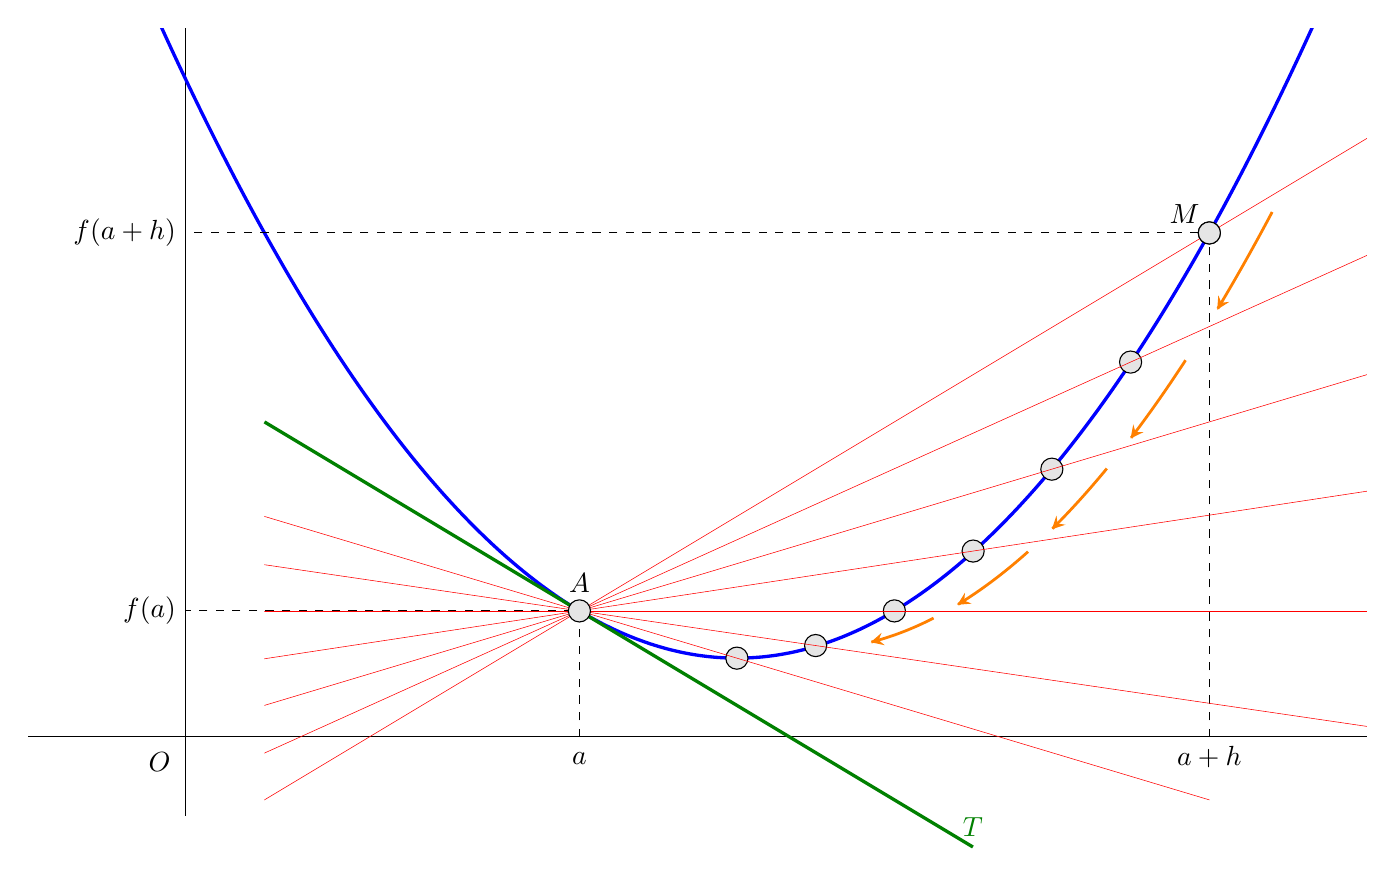
\begin{tikzpicture}[scale=2]
    
        \draw (-1,0) -- (7.5,0) (0,-.5) -- (0,4.5); % Axis
        \node[below left=2pt and 2pt] at (0,0) {$O$}; % Origin
        
        % Function curve        
        \begin{scope}       
            \clip (-1,0) rectangle (7.5,4.5);
            \draw[line width=1.2pt,color=blue,smooth,samples=100,domain=-2.5:7.5] plot(\x,{0.3*((\x)-3.5)*((\x)-3.5)+0.5}); 
        \end{scope}
        
        \def\xA{2.5} \def\yA{0.8}
        \coordinate (A) at (\xA,\yA);
        \draw[dashed] (\xA,0) node[below=2pt] {$a$} -- (A) -- (0,\yA) node[left] {$f(a)$};
                
        \def\xM{6.5} \def\yM{3.2}
        \coordinate (M) at (\xM,\yM);
        \draw[dashed] (\xM,0) node[below] {$a+h$} -- (M) -- (0,\yM) node[left] {$f(a+h)$};
        \begin{scope}       
            \clip (0.5,-0.5) rectangle (7.5,4.5);

            % Series of lines all through point A
            \foreach \xN/\yN in {6.5/3.2,6/2.38,5.5/1.7,5/1.18,4.5/0.8,4/0.58,3.5/0.5}
                {
                \coordinate (N) at (\xN,\yN);
                \tkzDrawPoint[size=8](N)
                \tkzDrawLine[add=2 and 3,color=red](A,N)
                }   
        \end{scope}
        
        \draw[line width=1.2pt,color=green!50!black,smooth,samples=100,domain=0.5:5] plot(\x,{-0.6*(\x)+2.3}) node[above] {$T$};            
        
        \tkzDrawPoints[size=8](A,M)
        \tkzLabelPoint[above=3pt](A){$A$}
        \tkzLabelPoint[above left](M){$M$}
        
        %%%%Arrows alongside the curve
        \foreach \a/\b in {6.55/6.9, 6/6.35, 5.5/5.85, 4.9/5.35, 4.35/4.75}
            {
            \draw[<-,>=stealth,line width=1pt,color=orange,smooth,samples=100,domain=\a:\b] plot(\x,{0.32*((\x)-3.95)*((\x)-3.95)+0.55});
            }
        
    \end{tikzpicture}
\end{remark}
\begin{proposition}
Note that $f'(a)$ is also equal to \[
\lim_{h\to 0} \frac{f(a + h) - f(a)}{h}
\]
by letting $x = a+ h$ so $h = x- a$.
\end{proposition}
\begin{example}
Let $f(x) = x^2$.
Then \begin{align*}
    f'(2) &= \lim_{x\to 2}\frac{f(x) - f(2)}{x-2}\\
    &= \lim_{x\to 2}\frac{x^2 - 4}{x-2}\\
    &= \lim_{x\to 2}\frac{(x-2)(x+2)}{x-2}\\
    &= \lim_{x\to 2}x+2\\
    &= 4 \tag{Since $f$ is cts.}\\
\end{align*}
In fact, \begin{align*}
    f'(a) &= \lim_{x\to a}\frac{f(x) - f(a)}{x-a}\\
    &= \lim_{x\to a}\frac{x^2 - a^2}{x-a}\\
    &= \lim_{x\to a}\frac{(x-a)(x+a)}{x-a}\\
    &= \lim_{x\to a}x+a\\
    &= 2a \tag{Since $f$ is cts.}\\
\end{align*}
So if $f(x) = x^2$, then $f'(x) = 2x$.
\end{example}
\begin{example}
Let $f(x) = x^2$. Then for $a > 0$,
\begin{align*}
    f'(a) &= \lim_{x\to a}\frac{\sqrt{x} - \sqrt{a}}{x-a}\\
    &= \lim_{x\to a}\frac{1}{\sqrt{x} + \sqrt{a}} \tag{Rationalize the Numerator}\\
    &= \frac{1}{2\sqrt{a}}\\
\end{align*}
Suppose $a = 0$, then \begin{align*}
    f'(a) &= \lim_{x\to 0^+}\frac{\sqrt{x} - 0}{x-0}\\
    &= \lim_{x\to a}\frac{1}{\sqrt{x}}\\
    &= \infty
\end{align*}
Thus $f'(x)$ is not differentiable at $x - 0$.
\end{example}
\subsection{Limit Laws}
\begin{cthm}[Derivative of a constant]
Let $f(x) = c$ be a constant function. Then $f'(x) = 0$.
\end{cthm}
\begin{proof}
    Let $a \in \R$. Then \begin{align*}
        f'(a) &= \lim_{x\to a} \frac{f(x) - f(a)}{x-a}\\
        &= \lim_{x\to a} \frac{c-c}{x-a}\\
        &= 0
    \end{align*}
\end{proof}
\begin{cthm}[Power Rule v1]
Let $n \in \N$. Consider $f(x) = x^n$ on $\R$. Then $f'(x) = nx^{n-1}$.
\end{cthm}
\begin{proof}
    Let $a \in \R$. Then, \begin{align*}
        f'(a) &= \lim_{x\to a} \frac{f(x) - f(a)}{x-a}\\
        &= \lim_{x\to a} \frac{x^n - a^n}{x-a}\\
        &= \lim_{x\to a} \frac{(x-a)(x^{n-1} + ax^{n-2} + \dots + a^{n-1})}{x-a}\\
        &= \lim_{x\to a} (x^{n-1} + ax^{n-2} + \dots + a^{n-1})\\
        &= a^{n-1} + a^{n-1} + \dots \tag{polynomials are cts.}\\
        &= na^{n-1}\\
    \end{align*}
    Note $n$ sweeps from $n-1$ to $0$, so $n$ terms in total.
\end{proof}
\begin{cthm}[Theorem 28.3]
Let $f$ and $g$ be differentiable at $a$. Let $c$ be a constant. Then $cf, f+g, fg, f/g$ (with $g(a) \neq 0$) are diff. at $a$.

They have the following derivatives:
\begin{enumerate}
    \item $(cf)'(a) = cf'(a)$
    \item $(f+g)'(a) = f'(a) + g'(a)$
    \item $(fg)'(a) = f'(a)g(a) + f(a)g'(a)$
    \item $(\frac{f}{g})'(a) = \frac{f'(a)g(a) - f(a)g'(a)}{g(a)^2} $
\end{enumerate}
\end{cthm}
\begin{proof}
    \begin{align*}
        (cf)'(a) &= \lim_{x\to a}\frac{(cf)(x) - (cf)(a)}{x-a}\\
        &= \lim_{x\to a}\frac{cf(x) - cf(a)}{x-a}\\
        &= c\lim_{x\to a}\frac{f(x) - f(a)}{x-a}\\
        &= cf'(a)
    \end{align*}
    \begin{align*}
        (f + g)'(a) &= \lim_{x\to a}\frac{(f+g)(x) - (f+g)(a)}{x-a}\\
        &= \lim_{x\to a}\frac{f(x)+g(x) - f(a)-g(a)}{x-a}\\
        &= \lim_{x\to a}\frac{f(x)f(a)}{x-a} + \lim_{x\to a} \frac{g(x) - g(a)}{x-a}\\
        &= f'(a) + g'(a)
    \end{align*}
    \begin{align*}
        (fg)'(a) &= \lim_{x\to a}\frac{(fg)(x) - (fg)(a)}{x-a}\\
        &= \lim_{x\to a}\frac{f(x)g(x) - f(a)g(a)}{x-a}\\
        &= \lim_{x\to a}\frac{f(x)g(x) - f(a)g(x) + f(a)g(x) - f(a)g(a)}{x-a}\\
        &= \lim_{x\to a}\frac{g(x)(f(x) - f(a)) + f(a)(g(x) - g(a))}{x-a}\\
        &= (\lim_{x\to a}g(x))\left(\lim_{x\to a}\frac{f(x)-f(a)}{x-a}\right) + (\lim_{x\to a}\frac{f(a) (g(x) - g(a))}{x-a})\\
        &= f'(a)g(a) + f(a)g'(a)\\
    \end{align*}
\end{proof}
\begin{example}
    Prove that $f(x) = |x|$ is not differentiable at $x=0$. Consider the left and right hand limits. 
    \begin{align*}
        \lim_{x\to 0^-} \frac{f(x) - f(0)}{x-0} &= \lim_{x\to 0^-} \frac{|x|}{x}\\
        &= \lim_{x\to 0^-} \frac{-x}{x}\\
        &= -1\\
        \\
        \lim_{x\to 0^+} \frac{f(x) - f(0)}{x-0} &= \lim_{x\to 0^+} \frac{|x|}{x}\\
        &= \lim_{x\to 0^+} \frac{x}{x}\\
        &= 1
    \end{align*}
    Thus the derivative does not exist at $x=0$.
\end{example}
\begin{cthm}[Theorem 28.2]
    If $f$ is differentiable at $a$, then $f$ is cts. at $a$.
\end{cthm}
\begin{proof}
    Suppose $f$ is differentiable at $a$, so that $\lim_{x\to a}\frac{f(x) - f(a)}{x-a}$ exists and is finite.
    We have \begin{align*}
        \lim_{x\to a}f(x) &= \lim_{x\to a} \left( (x-a)\left(\frac{f(x) - f(a)}{x-a}\right) + f(a)\right) \tag{This is equal to $f(x)$}\\
        &= \lim_{x\to a} (x-a) \lim_{x\to a} \left( \frac{f(x) - f(a)}{x-a}\right) + \lim_{x\to a} f(a)\\
        &= 0 \cdot f'(x) + f(a)\\
        &= f(a)
    \end{align*}
\end{proof}
\begin{proof}
    Now we can prove the Quotient Rule:
    \[
        \left(\frac{f}{g}\right)(a) = \frac{f'(a)g(a) - f(a)g'(a)}{(g(a))^2}
    \]
    for $g(a) \neq 0$.

    Since $g(a) \neq 0$ and $g(a)$ is a cts. function, $\exists I$ s.t. $a \in I$ for which $g(x) \neq 0 \forall x \in I$.

    For $x \in I$, we have \begin{align*}
        \left(\frac{f}{g}\right)(x) - \left(\frac{f}{g}\right)(a) &= \frac{f(x)}{g(x)} - \frac{f(a)}{g(a)}\\
        &= \frac{f(x)g(a) - f(a)g(x)}{g(x)g(a)}\\
        &= \frac{f(x)g(a) - g(a)f(a) + g(a)f(a) - f(a)g(x)}{g(x)g(a)}\\
        &= \frac{g(a)(f(x) - f(a)) - f(a)(g(x) - g(a))}{g(x)g(a)}
    \end{align*}
    Now we take the divide by $x-a$ and take the limit.
    \begin{align*}
        \lim_{x\to a} \frac{g(a)\frac{f(x) - f(a)}{x-a} - f(a)\frac{g(x) - g(a)}{x-a}}{g(x)g(a)} &= \frac{g(a)f'(x)- f(a)g'(x)}{g(x)g(a)} \tag{distribute the limits}\\
        &= \frac{f'(a)g(a) - f(a)g'(a)}{(g(a))^2} \tag{$g$ is cts.}
    \end{align*}
\end{proof}
\begin{cthm}[Power Rule v2]
    Let $m \in \N$ and consider $f(x) = x^{-m}$ for $x \neq 0$.

    Then $f(x) = \frac{1}{x^m} = \frac{g(x)}{h(x)}$ where $g(x) = 1$ and $h(x) = x^m$.
    Then, \begin{align*}
        f'(x) &= \frac{0(x^m) - 1(mx^{m-1}}{x^{2m}}\\
        &= \frac{-mx^{m-1}}{x^2m}\\
        &= =mx^{-m-1}
    \end{align*}
    Let $n = -m$, then $f'(x) = nx^{n-1}$
\end{cthm}
\begin{lemma}
    For $x \in \left( -\frac{\pi}{2}, \frac{\pi}{2}\right)$ and $x\neq 0$, we have \[
        \cos x \leq \frac{\sin x}{x} \leq 1
    \]
\end{lemma}
\begin{proof}
Consider the image for $0 < \alpha < \frac{\pi}{2}$.
    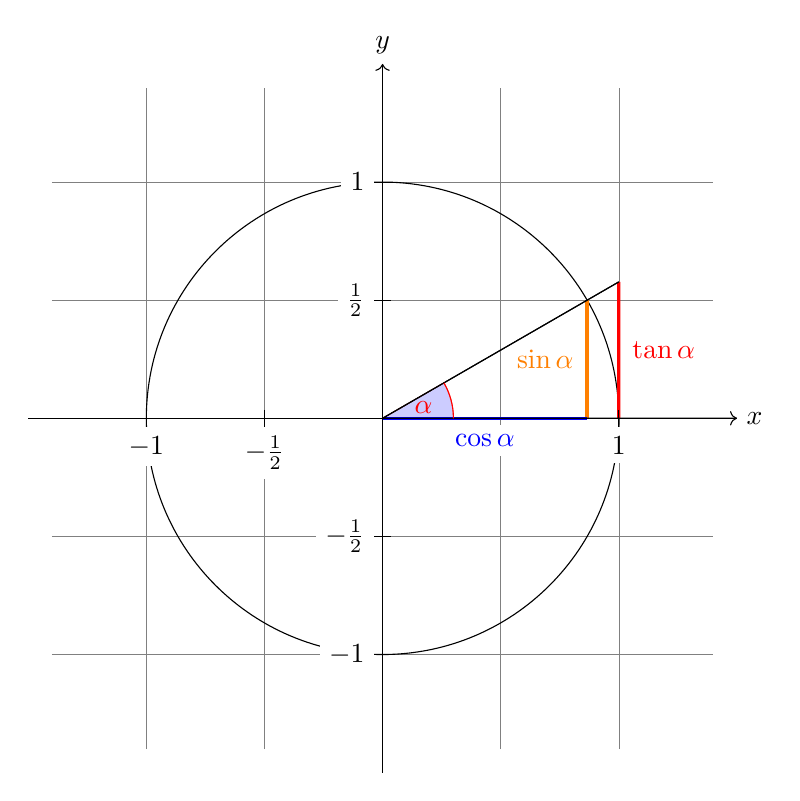
\begin{tikzpicture}[scale=3]

%grid lines
\draw[
        step=.5cm,
        gray,
        very thin
        ] 
        (-1.4,-1.4) grid (1.4,1.4);
\filldraw[
            fill=blue!20,
            draw=red!50
            ] 
            (0,0) -- (3mm,0mm)
arc [
        start angle=0, 
        end angle=30, 
        radius=3mm] 
        -- cycle;
%axes
\draw[->] (-1.5,0) -- (1.5,0) coordinate (x axis);
\draw[->] (0,-1.5) -- (0,1.5) coordinate (y axis);

%axes label
\node [right]at (1.5,0)(x){$x$};    
\node [above]at (0,1.5){$y$};

%circle 
\draw (0,0) circle [
                    radius=1cm
                    ];
                    
%triangle height
\draw[
        very thick,
        orange
        ]
        (30:1cm) -- node[
                        left=1pt,
                        fill=white
                        ] 
                        {$\sin \alpha$} (30:1cm |- x axis);
                        
%triangle base
\draw[
        very thick,
        blue
        ]
        (30:1cm |- x axis) -- node[
                                    below=2pt,
                                    fill=white
                                    ] 
                                    {$\cos \alpha$} (0,0);

%intersection
\path [name path=upward line] (1,0) -- (1,1);
\path [name path=sloped line] (0,0) -- (30:1.5cm);
\draw [name intersections={of=upward line and sloped line, by=t}]
        [very thick,red] 
        (1,0) -- node [right=1pt,fill=white]
        {$\displaystyle \tan \alpha $} (t);
\draw (0,0) -- (t);

%x-ticks
\foreach \x/\xtext in {-1, 
                        -0.5/-\frac{1}{2},
                                         1}
\draw (\x cm,1pt) -- (\x cm,-1pt) node[
                                        anchor=north,
                                        fill=white
                                        ] 
                                        {$\xtext$};
%y-ticks
\foreach \y/\ytext in {-1, 
                        -0.5/-\frac{1}{2}, 
                            0.5/\frac{1}{2}, 
                                            1}
\draw (1pt,\y cm) -- (-1pt,\y cm) node[
                                        anchor=east,
                                        fill=white
                                        ] 
                                        {$\ytext$};
%arc angle
\draw (x) coordinate (A)-- 
        (0,0) coordinate (B)-- 
            (t) coordinate (C)
pic [
        draw,
        red, 
        "$\alpha$",
        angle radius=9mm
        ] 
        {angle};
\end{tikzpicture}
    Let $A$ be the origin, $B$ be the point (1, 0), and $C$ the point where the hypotenuse touches the circle. (IDK how to graph)

    Then the area of triangle $ABC$ is: $\frac{1}{2}(1)(\sin \alpha) = \frac{\sin \alpha}{2}$.

    Since the circumference of the circle is $2\pi$, and the arc length of the slice is $\alpha$, the slice accounts for $\frac{\alpha}{2\pi}$ of the circumference of the circle. 

    Since the area of the circle is $\pi$, the area of the curve slice is $\left(\frac{\alpha}{2\pi}\right)(\pi) = \frac{\alpha}{2}$. 

    Also, the area of the large triangle is $\frac{1}{2}(1)(\tan \alpha) = \frac{1}{2}\tan \alpha$.

    Since \begin{align*}
        \text{area of ABC} &\leq \text{area of pie slice}\\
        &\leq \text{area of ABD}
    \end{align*} we have 
    \begin{align*}
        &\frac{1}{2}\sin x \leq \frac{x}{2} \leq \frac{1}{2} \tan x\\
        &\implies 0 < \sin x \leq x \leq \tan x\\
        &\implies \frac{\cos x}{\sin x} \leq \frac{1}{x} \leq \frac{1}{\sin x}\\
        &\implies \cos x \leq \frac{\sin x}{x} \leq 1
    \end{align*}

    For the negative part, since $\cos (-x) = \cos x$ and $\frac{\sin (-x)}{-x} = \frac{\sin x}{x}$, we can replace the $\alpha$ with its negation.
    
\end{proof}
\begin{theorem}
    \[\lim_{x\to 0}\frac{\sin x}{x} = 1\] and \[
    \lim_{x \to 0}\frac{\cos x - 1}{x}
    \] 
\end{theorem}
\begin{proof}
    For $-\frac{\pi}{2} < x < \frac{\pi}{2}$, we have $\cos x \leq \frac{\sin x}{x} \leq 1$. Since $\lim_{x\to 0}\cos x = 1$, by squeeze theorem $\lim_{x\to 0} \frac{\sin x}{x} x = 1$.

    Note that \begin{align*}
        \frac{\cos x - 1}{x} &= \frac{(\cos x - 1)(\cos x + 1)}{x(\cos x + 1)}\\
        &= \frac{\cos^2 x - 1}{x(\cos x + 1)}\\
        &= \frac{-\sin^2 x}{x(\cos x + 1)} \tag{Pythagorean Identity}\\
        &= \left(\frac{\sin x}{x}\right)\left(\frac{-\sin x}{x}\right)\\
    \end{align*}
    Taking limits, we have $\lim \left(\frac{\sin x}{x}\right)\left(\frac{-\sin x}{x}\right) = 1\left(\frac{-0}{2}\right) = 0$.
\end{proof}
\begin{theorem}
    $\sin x$ and $\cos x$ are differentiable on $\R$ with \[
        (\sin x)' = \cos x
    \] and \[
        (\cos x)' = -\sin x
    \]
\end{theorem}
\begin{proof}
    If $f(x) = \sin x$, then \begin{align*}
        f'(a) &= \lim_{h\to 0} \frac{\sin (a+h) - \sin a}{h}\\
        &= \lim_{h\to 0} \frac{\sin a\cos h +\cos a \sin h - \sin a}{h}\\
        &= \lim_{h\to 0} (\sin a)\left(\frac{\cos h - 1}{h}\right) + \cos a \left(\frac{\sin h}{h}\right)\\
        &= \sin a \lim_{h\to 0} \frac{\cos h -1}{h} + \cos a \frac{\sin h}{h}\\
        &= 0 + \cos a (1)\\
        &= \cos a
    \end{align*}
    If $f(x) = \cos x$, then \begin{align*}
        f'(a) &= \lim_{h\to 0} \frac{\cos (a+h) - \cos a}{h}\\
        &= \lim_{h\to 0} \frac{\cos a \cos h - \sin a \sin h - \cos a}{h}\\
        &= \lim_{h\to 0} \cos a \left(\frac{\cos h - 1}{h}\right) - \sin a\left( \frac{\sin h}{h}\right)\\
        &= \cos a (0) - \sin a (1)\\
        &= -\sin a
    \end{align*}
\end{proof}
\begin{corollary}
Now we can differentiate the other trig functions. For example, let $f(x) = \tan x$. Then, \begin{align*}
    h'(x) &= \frac{(\sin x)' \cos x - \sin x(\cos x)'}{\cos^2x}\\
    &= \frac{\cos^2x+\sin^2x}{\cos^2x}\\
    &= \sec^2 x
\end{align*}
\end{corollary}
\begin{cthm}[Theorem 28.4 (Chain Rule)]
    If $f$ is differentiable at $a$, and $g$ is differentiable at $f(a)$, then \[
    \left((g\circ f)(a)\right)' = g'(f(a))f'(a)
    \]
\end{cthm}
\begin{proof}
    Notice that \[
    \frac{(g \circ f)(x) - (g \circ f)(a)}{x-a} = \frac{g(f(x)) - g(f(a))}{f(x) - f(a)} \cdot \frac{f(x) - f(a)}{x-a}
    \]

    Can we use limits?
    We have \[
    \left(\lim_{x\to a}\frac{g(f(x)) - g(f(a))}{f(x)-f(a)}\right)\left(\lim_{x\to a} \frac{f(x) - f(a)}{x-a}\right)
    \]
    Since $f$ is cts. at $a$, we have $\lim_{x\to a} f(x) = f(a)$.

    Thus it looks like the limit is going to $g'(f(a)) f'(a)$.

    However, this proof doesn't work since we can be dividing by $0$ with $f(x) = f(a)$.

    (Full proof on brightspace)
\end{proof}
\begin{example}
    Let $f(x) = \sin (x^2 + x)$. Then, $f'(x) = \cos (x^2 + x) \cdot (2x + 1)$

    Let $f(x) = \big( \sin (x^2)\big)^2$. Then $f'(x) = 2\sin(x^2) \cdot \cos (x^2) \cdot 2x$

    Let $f(x) = x^2 \sin \left(\frac{1}{x}\right)$. Then $f'(x) = 2x(\sin \left(\frac{1}{x}\right)) + (x^2)(\cos \left(\frac{1}{x}\right)) \cdot (-x^{-2})$
\end{example}
\begin{cthm}[Theorem 29.1]
    Let $f$ be defined on an open interval $I$ containing $x_0$. Suppose $f$ assumes its max/min and $f$ is differentiable on $I$. Then, $f'(x_0) = 0$.
\end{cthm}
\begin{proof}
    Suppose $f$ is defined on $(a, b) = I$ with $x_0 \in I$. WLOG, assume $f$ hits its max at $x_0$. 

    If $f'(x_0) > 0$, then we have $f'(x_0) = \lim_{x\to x_0} \frac{f(x)-f(x_0)}{x-x_0} > 0$. Let $\ep = f'(x_0)$. Then $\exists \delta > 0$ s.t. $a < x_0 - \delta < x_0 < x_0 + \delta < b$ and 
    \[
    0 < \abs{x - x_0} < \delta \implies \abs{\frac{f(x) - f(x_0)}{x - x_0} - f'(x)} < f'(x_0) = \ep
    \]
    Thus \[
    -f(x_0) < \frac{f(x) - f(x_0)}{x- x_0} - f'(x_0) < f'(x_0)
    \]
    and so \[
    \frac{f(x) - f(x_0)}{x-x_0} > 0
    \]
    Taking $x_0 < x < x_0 + \delta$, we have \begin{align*}
        f(x) - f(x_0) &> 0\\
        f(x) &> f(x_0)
    \end{align*}
    This is a contradiction, since $f$ takes its max at $x_0$.

    Suppose $f'(x) < 0$. Let $\ep = -f(x_0)$, then $\exists \delta > 0$ s.t. \[
    0 < |x-x_0| < \delta \implies \abs{\frac{f(x) - f(x_0)}{x-x_0} - f'(x_0)} < f'(x_0) 
    \]
    Thus we have\[
    \frac{f(x) - f(x_0)}{x-x_0} < 0
    \]
    Taking $x_0 - \delta < x < x_0$ so that $x - x_0 < 0$, we have \begin{align*}
        f(x) - f(x_0) &> 0\\
        f(x) &> f(x_0)
    \end{align*}
    This is a contradiction, since $f$ takes its max at $x_0$.

    Thus we must have $f'(x) = 0$.
\end{proof}
\begin{corollary}
    Thus if we have a function on a closed interval, by Theorem 18.1, it must have a max/min and then $f$ can only hit those points at the endpoints, any non-differentiable points, or where the derivative is $0$.
\end{corollary}
\begin{example}
    Find the max and min of $f(x) = x^5 + x^4 - 5x^3 - x^2 + 8x - 4$ on $[-2, 2]$.

    Since polynomials are cts. everywhere, we only need to look at the endpoints and the derivative.

    We have $f'(x) = 5x^4 + 4x^3 - 15x^2 - 2x + 8$. By factor theorem and synthetic division, we have \[
    f'(x) = (x-1)^2(x+2)(5x+4)
    \]
    There are roots at $x=1, -2, -\frac{4}{5}$.

    Thus \begin{align*}
        f(-2) &= 0\\
        f(-\frac{4}{5}) &= \frac{-2^2 \cdot 3^8}{5^3}\\
        f(1) &= 0\\
        f(2) &= 16
    \end{align*}
    Thus the max and min are at $x=2, -\frac{4}{5}$
\end{example}
\begin{example}
    Find the max and min of $f(x) = x^{\frac{2}{3}}$ on $[-1, 1]$.

    We have $f'(x) = \frac{2}{3}x^{\frac{-1}{3}}$ when $x \neq 0$. For $x = 0$, it can be shown the limit does not exist.

    Thus we must check $x = 0$. Now we set $f'(x) = 0$. We have \[
    \frac{2}{3x^{\frac{1}{3}}} = 0
    \]
    This is never true. Thus there are no additional points to check.

    We have \begin{align*}
        f(1) &= 1\\
        f(0) &= 0\\
        f(-1) &= 1
    \end{align*}
\end{example}
\subsection{Mean Value Theorem}
\begin{cthm}[Theorem 29.2 (Rolle's Theorem)]
    Let $f$ be cts. on $[a, b]$, differentiable on $(a, b)$. Suppose $f(a) = f(b)$. Then $\exists x \in (a, b)$ s.t. $f'(x) = 0$.
\end{cthm}
\begin{proof}
    By 18.1, $\exists x_0, y_0 \in [a,b]$ s.t. $f(x_0) \leq f(x) \leq f(y_0) \forall x \in [a,b]$. 

    If $x_0, y_0$ are the endpoints, then $f$ is a constant function on the interval since $f(x_0) = f(y_0)$ and so $f'(x) = 0 \forall x$.

    Otherwise, $f$ assumes a max/min at $x \in (a, b)$ and so by Theorem 29.1, $f'(x) = 0$.
\end{proof}
\begin{cthm}[Theorem 29.3 (Mean Value Theorem)]
    Let $f$ be cts. on $[a, b]$ and differentiable on $(a, b)$, then $\exists x \in (a, b)$ such that $f'(x) = \frac{f(b) - f(a)}{b-a}$. This is the average rate of change between $a$ and $b$, and the slope of the secant line, but $f'(x)$ is the instantaneous rate of change at $x$, and the slope of the tangent line.
\end{cthm}
\begin{proof}
    Let $L(x)$ be the function whose graph is a straight line connecting $(a, f(a))$ and $(b, f(b))$ (secant line). Thus $L(a) = f(a)$ and $L(b) = f(b)$. Furthermore, $L'(x) = \frac{f(b) - f(a)}{b-a}$ for all $x$. 

    Let $g(x) = f(x) - L(x)$ for $x \in [a, b]$. It follows that $g$ is cts. on $[a, b]$, diff. on $(a, b)$, and $g(a) = 0 = g(b)$. By Rolle's Theorem, there is $x \in (a, b)$ with $g'(x) = 0$. Since $g'(x) = f'(x) - L'(x)$, we have $f'(x) = L'(x)$, or \[
    f'(x) = \frac{f(b) - f(a)}{b-a}
    \] 
\end{proof}
\begin{corollary}
    (29.4)

    Let $f$ be differentiable on $(a, b)$, with $f'(x) = 0 \forall x \in (a, b)$. Then $f$ must be constant on $(a, b)$.
\end{corollary}
\begin{proof}
    Suppose $f'(x) = 0$ on $(a, b)$ but $f$ is not constant. Then there are $x_1, x_2 \in (a, b)$ and with $x_1 < x_2$, where $f(x_1) \neq f(x_2)$. By the MVT, there is $x \in (x_1, x_2)$, with $f'(x) = \frac{f(x_2) - f(x_1)}{x_2 - x_1} \neq 0$, a contradiction.
\end{proof}
\begin{corollary}
    (29.5)
    Let $f, g$ be diff. on $(a, b)$ that have the same derivative, i.e. $f' = g'$ on $(a, b)$. Then there is a constant $c$ such that $f(x) = g(x) + c$ for all $x \in (a, b)$. 
\end{corollary}
\begin{proof}
    Let $h = f-g$, then $h' = f' - g' = 0$. By previous corollary, $h$ is constant on $(a, b)$.
\end{proof}
\begin{example}
    Find all functions whose derivative is $x^2$.

    We can find $\frac{1}{3}x^3$ by inspection. Thus $\frac{1}{3}x^3 + c$ will have derivative $x^2$ for any constant $c$. By previous corollary, no other such functions can unique.
\end{example}
\begin{definition}
    Let $f$ be defined on $I$. 
    
    $f$ is \textbf{strictly increasing} on $I$ if $x_1, x_2 \in I$ with $x_1 < x_2$ imply $f(x_1) < f(x_2)$.

    $f$ is \textbf{increasing} on $I$ if $x_1, x_2 \in I$ with $x_1 < x_2$ imply $f(x_1) \leq f(x_2)$.
    
    $f$ is \textbf{strictly decreasing} on $I$ if $x_1, x_2 \in I$ with $x_1 < x_2$ imply $f(x_1) > f(x_2)$.

    $f$ is \textbf{decreasing} on $I$ if $x_1, x_2 \in I$ with $x_1 < x_2$ imply $f(x_1) \geq f(x_2)$.
\end{definition}
\begin{corollary}
    (29.7)

    Let $f$ be diff. on $(a, b)$. Then 
    \begin{enumerate}
        \item $f$ is strictly increasing on $(a, b)$ if $f'(x) > 0$ on $(a, b)$.
        \item $f$ is increasing on $(a, b)$ if $f'(x) \geq 0$ on $(a, b)$.
        \item $f$ is strictly decreasing on $(a, b)$ if $f'(x) < 0$ on $(a, b)$.
        \item $f$ is decreasing on $(a, b)$ if $f'(x) \leq 0$ on $(a, b)$.
    \end{enumerate}
\end{corollary}
\begin{proof}
    Proof of 3:

    Consider $x_1, x_2 \in (a, b)$ with $x_1 < x_2$. By MVT, there is $x \in (x_1, x_2)$ with $\frac{f(x_2) - f(x_1)}{x_2 - x_1} = f'(x) < 0$.
    Thus $f(x_2) - f(x_1) < 0$ and so $f(x_1) > f(x_2)$.

    Proof of others is almost identical.
\end{proof}
\subsection{Inverse Functions}
\begin{definition}
    A function $f: A \to B$ is \textbf{injective}, or one-to-one, if for all $x, y \in A$, then $f(x) = f(y) \implies x = y$.
\end{definition}
\begin{exercise}
    If $f$ is strictly increasing or decreasing, then $f$ is injective.
\end{exercise}
\begin{remark}
    If $f: A \to \range f$ is injective, then $f$ is invertible. There exists a function $f^{-1}: \range f \to A$ such that $(f \circ f^{-1})(x) = x$ and $(f^{-1} \circ f)(x) = x$ for all $x$.
\end{remark}
\begin{cthm}[Theorem 29.9]
    If $f$ is injective and cts. on $I$, and differentiable at $x_0 \in I$, then $f^{-1}$ is cts. on $I$ and diff. at $f(x_0)$ except $f'(x_0) \neq 0$.
\end{cthm}
\begin{remark}
    What is $(f^{-1})'(y_0)$?

    Since $(f^{-1} \circ f)(x) = x$ for all $x \in A$, so $(f^{-1} \circ f)'(x)= 1$. Thus $1 = (f^{-1}(f(x)))' = (f^{-1})'(f(x)) \circ f'(x)$.
    
    Thus $1 = (f^{-1})'(f(x_0))f'(x_0)$, so \[
    (f^{-1})'(y_0) = \frac{1}{f'(x_0)} = \frac{1}{f'(f^{-1}(y_0))}
    \]
\end{remark}
\begin{example}
    Let $n \in \N$. Consider $g(x) = x^{\frac{1}{n}}$. 
    \[
    \dom g = \begin{cases}
        [0, \infty) &\text{if $n$ is even}\\
        \R &\text{if $n$ is odd}\\
    \end{cases}
    \]
    It can be shown that $g$ is cts. on its domain and $g$ is injective.

    Thus $g^{-1} = f$ exists, for $f(x) = x^n$. We know $f'(x) = nx^{n-1}$. Also $f^{-1} = g$.

    Let $y_0 \in \dom g$. Then $g'(y_0) = (f^{-1})'(y_0) = \frac{1}{n(y_0^{\frac{1}{n}})^{n-1}} = \frac{1}{ny_0^{\frac{n-1}{n}}} = \frac{1}{n}y_0^{\frac{1}{n} - 1}$.
\end{example}
\begin{cthm}[Power Rule v3]
    Now suppose $F(x) = x^{\frac{m}{n}}$ for $m, n \in \Z, n > 0$.

    Then $F = h \circ g$ for $h(x) = x^m$ and $g(x) = x^{\frac{1}{n}}$. We know $h'(x) = mx^{m-1}$ and $g'(x) = \frac{1}{n}x^{\frac{1}{n} - 1}$. Thus $F'(x) = m(x^{\frac{1}{n}})^{m-1} (\frac{1}{n}x^{\frac{1}{n} - 1} = \frac{m}{n}x^{\frac{m}{n} -1}$

    Let $r \in Q$. Then the derivative of $x^r$ is $rx^{r-1}$ where defined.
\end{cthm}
\subsection{Trig Functions}
\begin{example}
    $f(x) = \sin x$ is injective on $[-\frac{\pi}{2}, \frac{\pi}{2}]$ with range $[-1, 1]$.

    We write $f^{-1}(x) = \arcsin x$ or $f^{-1}(x) = \sin^{-1}x$.

    We know $f'(x) = \cos x$. Let $y_0 \in [-1, 1]$. If $x_0 = \arcsin y_0$, then $y_0 = \sin x_0$. \[
    (\arcsin)'(y_0) = \frac{1}{\cos x_0} = \frac{1}{\sqrt{1 - y_0^2}}
    \]
    since $\cos x_0 = \sqrt{1 - \sin^2 x_0}$.

    Thus the derivative of $\arcsin x$ is $\frac{1}{\sqrt{1 - x^2}}$.
\end{example}
\end{document}
